\chapter{Análisis Experimental} \label{capitulo:analisis-experimental}
\markright{Análisis Experimental}

En este capitulo se presentan las decisiones tomadas en torno a las configuraciones de los clasificadores y los resultados obtenidos durante los experimentos y su análisis. 

\section{Decisiones de configuración} \label{capitulo:configuracion}

\paragraph{} Durante el análisis experimental fueron realizadas comparaciones entre las clasificaciones obtenidas por redes neuronales y SVM.
En particular, fue de interés estudiar el comportamiento de las redes neuronales y SVM en términos del tamaño del problema.

\paragraph{} Tomando el trabajo de \citet{savant-original} como inspiración, se optó por trabajar con clasificadores entrenados con una determinada dimensión del problema (en particular $512$ tareas sobre $16$ máquinas o $512\times 16$) a la hora de clasificar instancias del problema de menor, igual y mayor cantidad de tareas.
Para hacer esto posible, se generaron instancias del problema de dimensión $512\times 16$, utilizadas para el entrenamiento de los clasificadores.
Así también, para cada dimensión del problema desde $17\times 16$ hasta $1024\times 16$, se generaron conjuntos de $10$ instancias del problema, las cuales fueron utilizadas para calcular y comparar la precisión en la clasificación para redes neuronales y SVM.

\paragraph{} Las redes neuronales fueron entrenadas con diferentes cantidades de capas ocultas, habiéndose generado con $2$, $3$ y $4$ capas ocultas, siendo 4 el máximo de capas ocultas empleado debido a limitaciones de recursos y tiempos de entrenamiento altos.

\paragraph{} Como fue mencionado en el capítulo \textit{Implementación}, para obtener una primera selección de parámetros de configuración para el entrenamiento de las redes neuronales se utilizó la clase \textit{model\_selection.GridSearchCV} de \textit{scikit-learn}.
Este método realiza una búsqueda, mediante validación cruzada, de los mejores parámetros para el entrenamiento de un clasificador.
Para eso es necesario definir conjuntos de posibles valores a ser utilizados en los parámetros de los clasificadores.
Entre los valores de los parámetros que se seleccionaron para utilizar el método \textit{GridSearchCV} con las redes neuronales, se encuentran: \textit{lbfgs}, \textit{sgd}, \textit{adam} para el parámetro \textit{solver}; \textit{1e-2} y \textit{1e-4} para el coeficiente de aprendizaje llamado \textit{alpha} y \textit{relu}, \textit{tanh} e \textit{identity} como funciones de activación para el parámetro \textit{activation}.
Los resultados del método \textit{GridSearch()} para los parámetros mencionados se muestran en el Cuadro \ref{table:parametros}.
Con respecto al parámetro \textit{activation} se observó que el valor seleccionado por el método \textit{GridSearch()} fue \textit{relu}; esto fue de particular interés debido a que dicha función de activación cambia de forma abrupta en su pendiente y estudios tempranos demostraron resultados poco prometedores que, al variar la función de activación, mejoraban notoriamente.
Esto llevó a variar las funciones de activación para probar además el comportamiento de las redes neuronales con funciones de activación con pendientes que no tuvieran cambios abruptos.
El resto de los parámetros se mantuvieron de acuerdo a los resultados del método \textit{GridSearch()}.
\\

\begin{table}[h!]

\centering
\begin{tabular}{ |p{0.25\linewidth}|p{0.25\linewidth}| } 
\hline
\textbf{Parámetro} & \textbf{Valor}\\
\hline
solver & lbfgs\\ 
\hline
alpha & 1e-2\\ 
\hline
activation & relu\\ 
\hline
\end{tabular}
\caption{ Valores para los parámetros de las redes neuronales, obtenidos mediante el método \textit{GridSearch() de la biblioteca \textit{scikit-learn}}}
\label{table:parametros}
\end{table}

\paragraph{}  Se evaluaron las redes neuronales resultantes de las combinaciones de las funciones de activación \textit{relu}, \textit{tanh} e \textit{identity} y las cantidades de capas ocultas, profundizando en las pruebas para aquellas combinaciones que mostraban resultados más prometedores.

\section{Análisis combinado para redes neuronales de 2, 3 y 4 capas ocultas}

\paragraph{}En primer lugar fueron comparados los resultados de \textit{makespan} para soluciones obtenidas a partir de las redes neuronales, utilizando como funciones de activación a \textit{tanh}, \textit{identity} y \textit{relu}, con 2, 3 y 4 capas ocultas.
Así mismo, en esta comparación también fueron analizados los resultados SVM. 

\paragraph{} Cada clasificador fue entrenado con 100 instancias del problema de dimensión $512\times16$, lo que se traduce en 512000 instancias de entrenamiento para los clasificadores. 

\paragraph{} Para cada dimensión del rango estudiado, se utilizaron 10 instancias del problema para validar el rendimiento de dichos clasificadores, y los resultados mostrados son un promedio de estas.

\paragraph{} Fueron identificados aquellos clasificadores que obtuvieron mejores resultados en \textit{makespan}.
Las figuras \ref{fig:relu234}, \ref{fig:identity234} y \ref{fig:tanh234} muestran las diferencias de \textit{makespan} porcentuales con respecto al \textit{makespan} obtenido por el algoritmo Min-Min, para la clasificación de instancias del problema en un rango de dimensiones que va desde $17\times16$ a $1024\times16$.

\paragraph{} De manera similar, los resultados también fueron agrupados de acuerdo a su dimensión.
Esta agrupación fue realizada de a 200 tareas con la excepción de que el primero y último de los conjuntos van desde la dimensión $17\times16$ a $200\times16$ y $1000\times16$ a $1024\times16$ respectivamente.

\paragraph{}La Figura \ref{fig:relu234} muestra los resultados para las redes neuronales utilizando la función de activación \textit{relu}.
En dicha Figura se observa que el \textit{makespan} generado por los resultados de la SVM se aproxima más al \textit{makespan} dado por los resultados del algoritmo Min-Min que para los resultados obtenidos con las redes neuronales, cualquiera sea la cantidad de capas ocultas utilizada. 

\paragraph{} Cabe destacar que a medida que aumenta la cantidad de capas ocultas de la red neuronal, los resultados se alejan de los valores esperados llegando, para clasificaciones sobre dimensiones pequeñas, a estar a más del $100\%$ por sobre los valores esperados.
Los mejores resultados de las redes neuronales se observan para aquellas redes neuronales con dos capas ocultas.
% TODO ¿agregar algo sobre que probablemente la función aprendida no requiere de la complejidad que permite una mayor cantidad de capas ocultas? 


\begin{figure}[H]
  \centering
  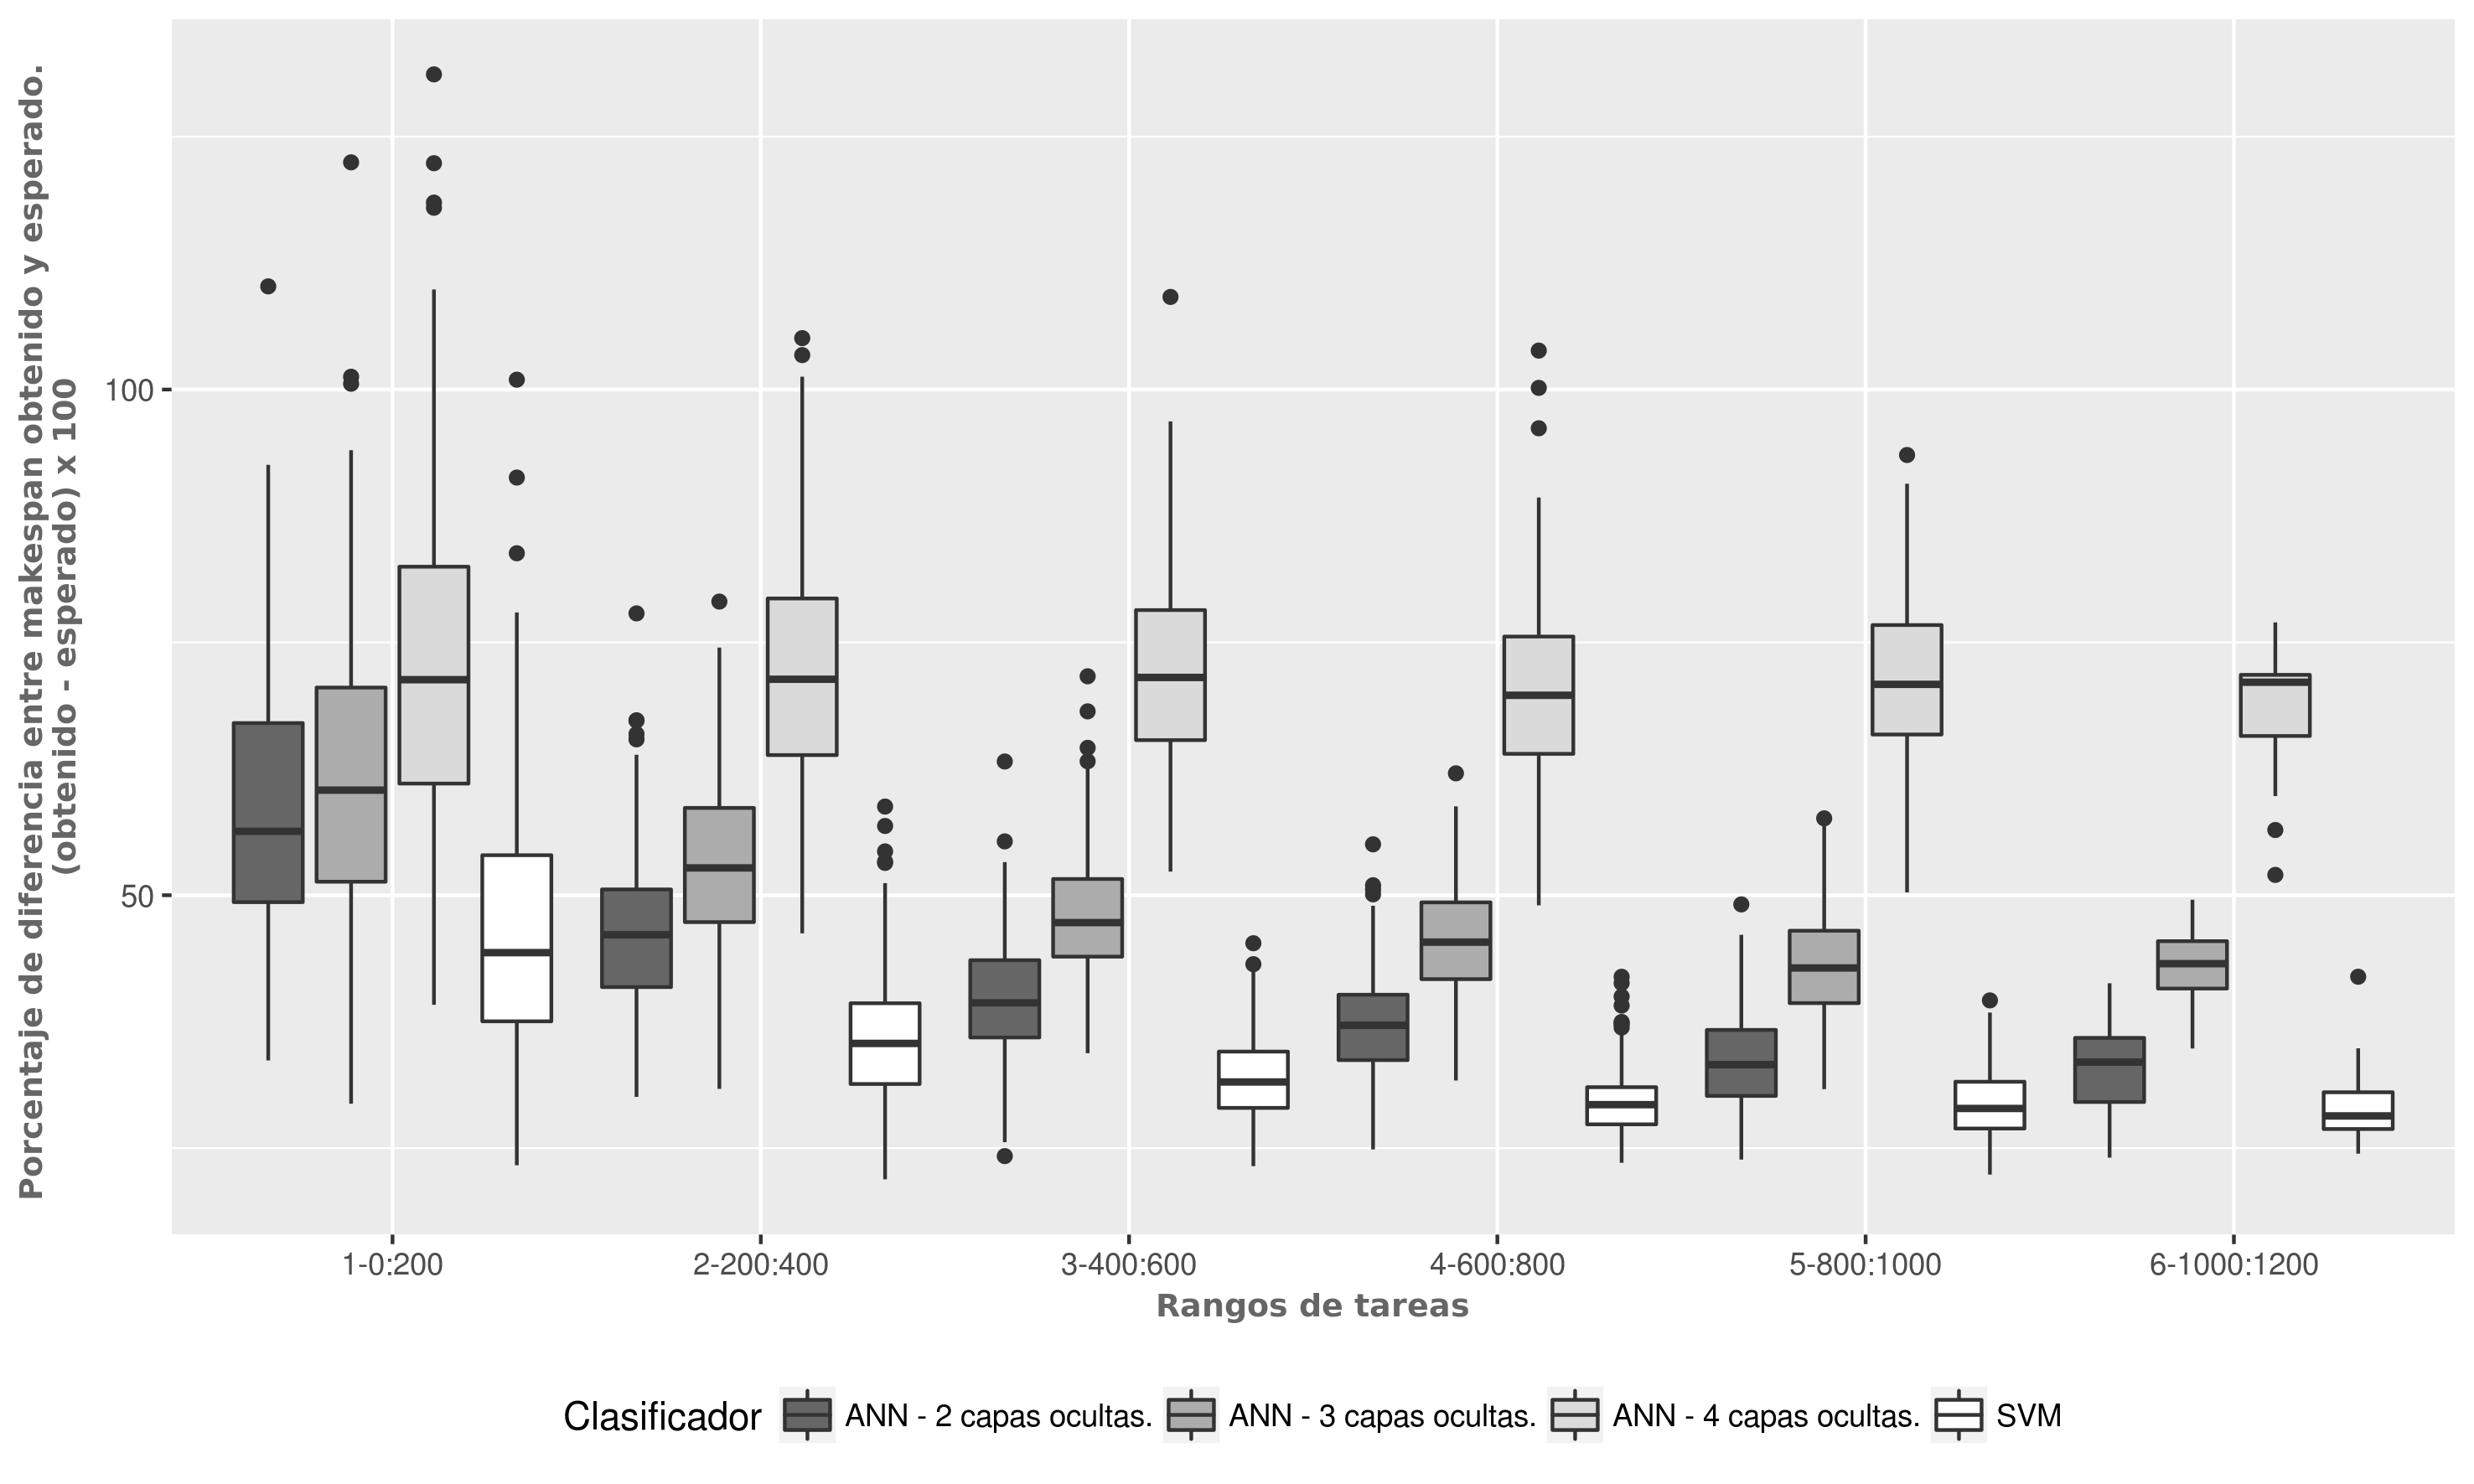
\includegraphics[width=\columnwidth]{imagenes/comparacion_anns_relu.png}
  \caption{Comparación de  la diferencia porcentual  de los resultados de \textit{makespan} para redes neuronales con función de activación \textit{relu}, con respecto al \textit{makespan} obtenido por el algoritmo Min-Min.
Se comparan redes neuronales de 2, 3 y 4 capas ocultas.
Así también se muestran los resultados obtenidos con el algoritmo de SVM.}
  \label{fig:relu234}
\end{figure}

\paragraph{}La Figura \ref{fig:identity234} muestra los resultados para las redes neuronales utilizando la función de activación \textit{identity}.
En este caso los resultados para las redes neuronales son más próximos a los valores esperados dados por el algoritmo Min-Min que los resultados dados por SVM.
Ya desde tareas de dimensión $ 200 \times 16$ se comienzan a observar mejoras en el \textit{makespan}, siendo aún más evidentes para instancias del problema de dimensión mayor.
Nuevamente se observa que los resultados más próximos al \textit{makespan} esperado están dados por la red neuronal con dos capas ocultas. 

\paragraph{}En la Figura \ref{fig:tanh234} se observan los resultados para las redes neuronales utilizando la función de activación \textit{tanh}.
En este caso, la red neuronal con dos capas ocultas mejora los resultados obtenidos a partir de instancias del problema de dimensión $ 400 \times 16$ en adelante. 

\paragraph{}En los casos presentados en las figuras \ref{fig:relu234}, \ref{fig:identity234} y \ref{fig:tanh234}, los mejores resultados de las redes neuronales se encuentran para aquellas de dos capas ocultas.
En éstas fue profundizado el estudio de cara a entender mejor la naturaleza de las soluciones generadas. 

\begin{figure}[H]
  \centering
  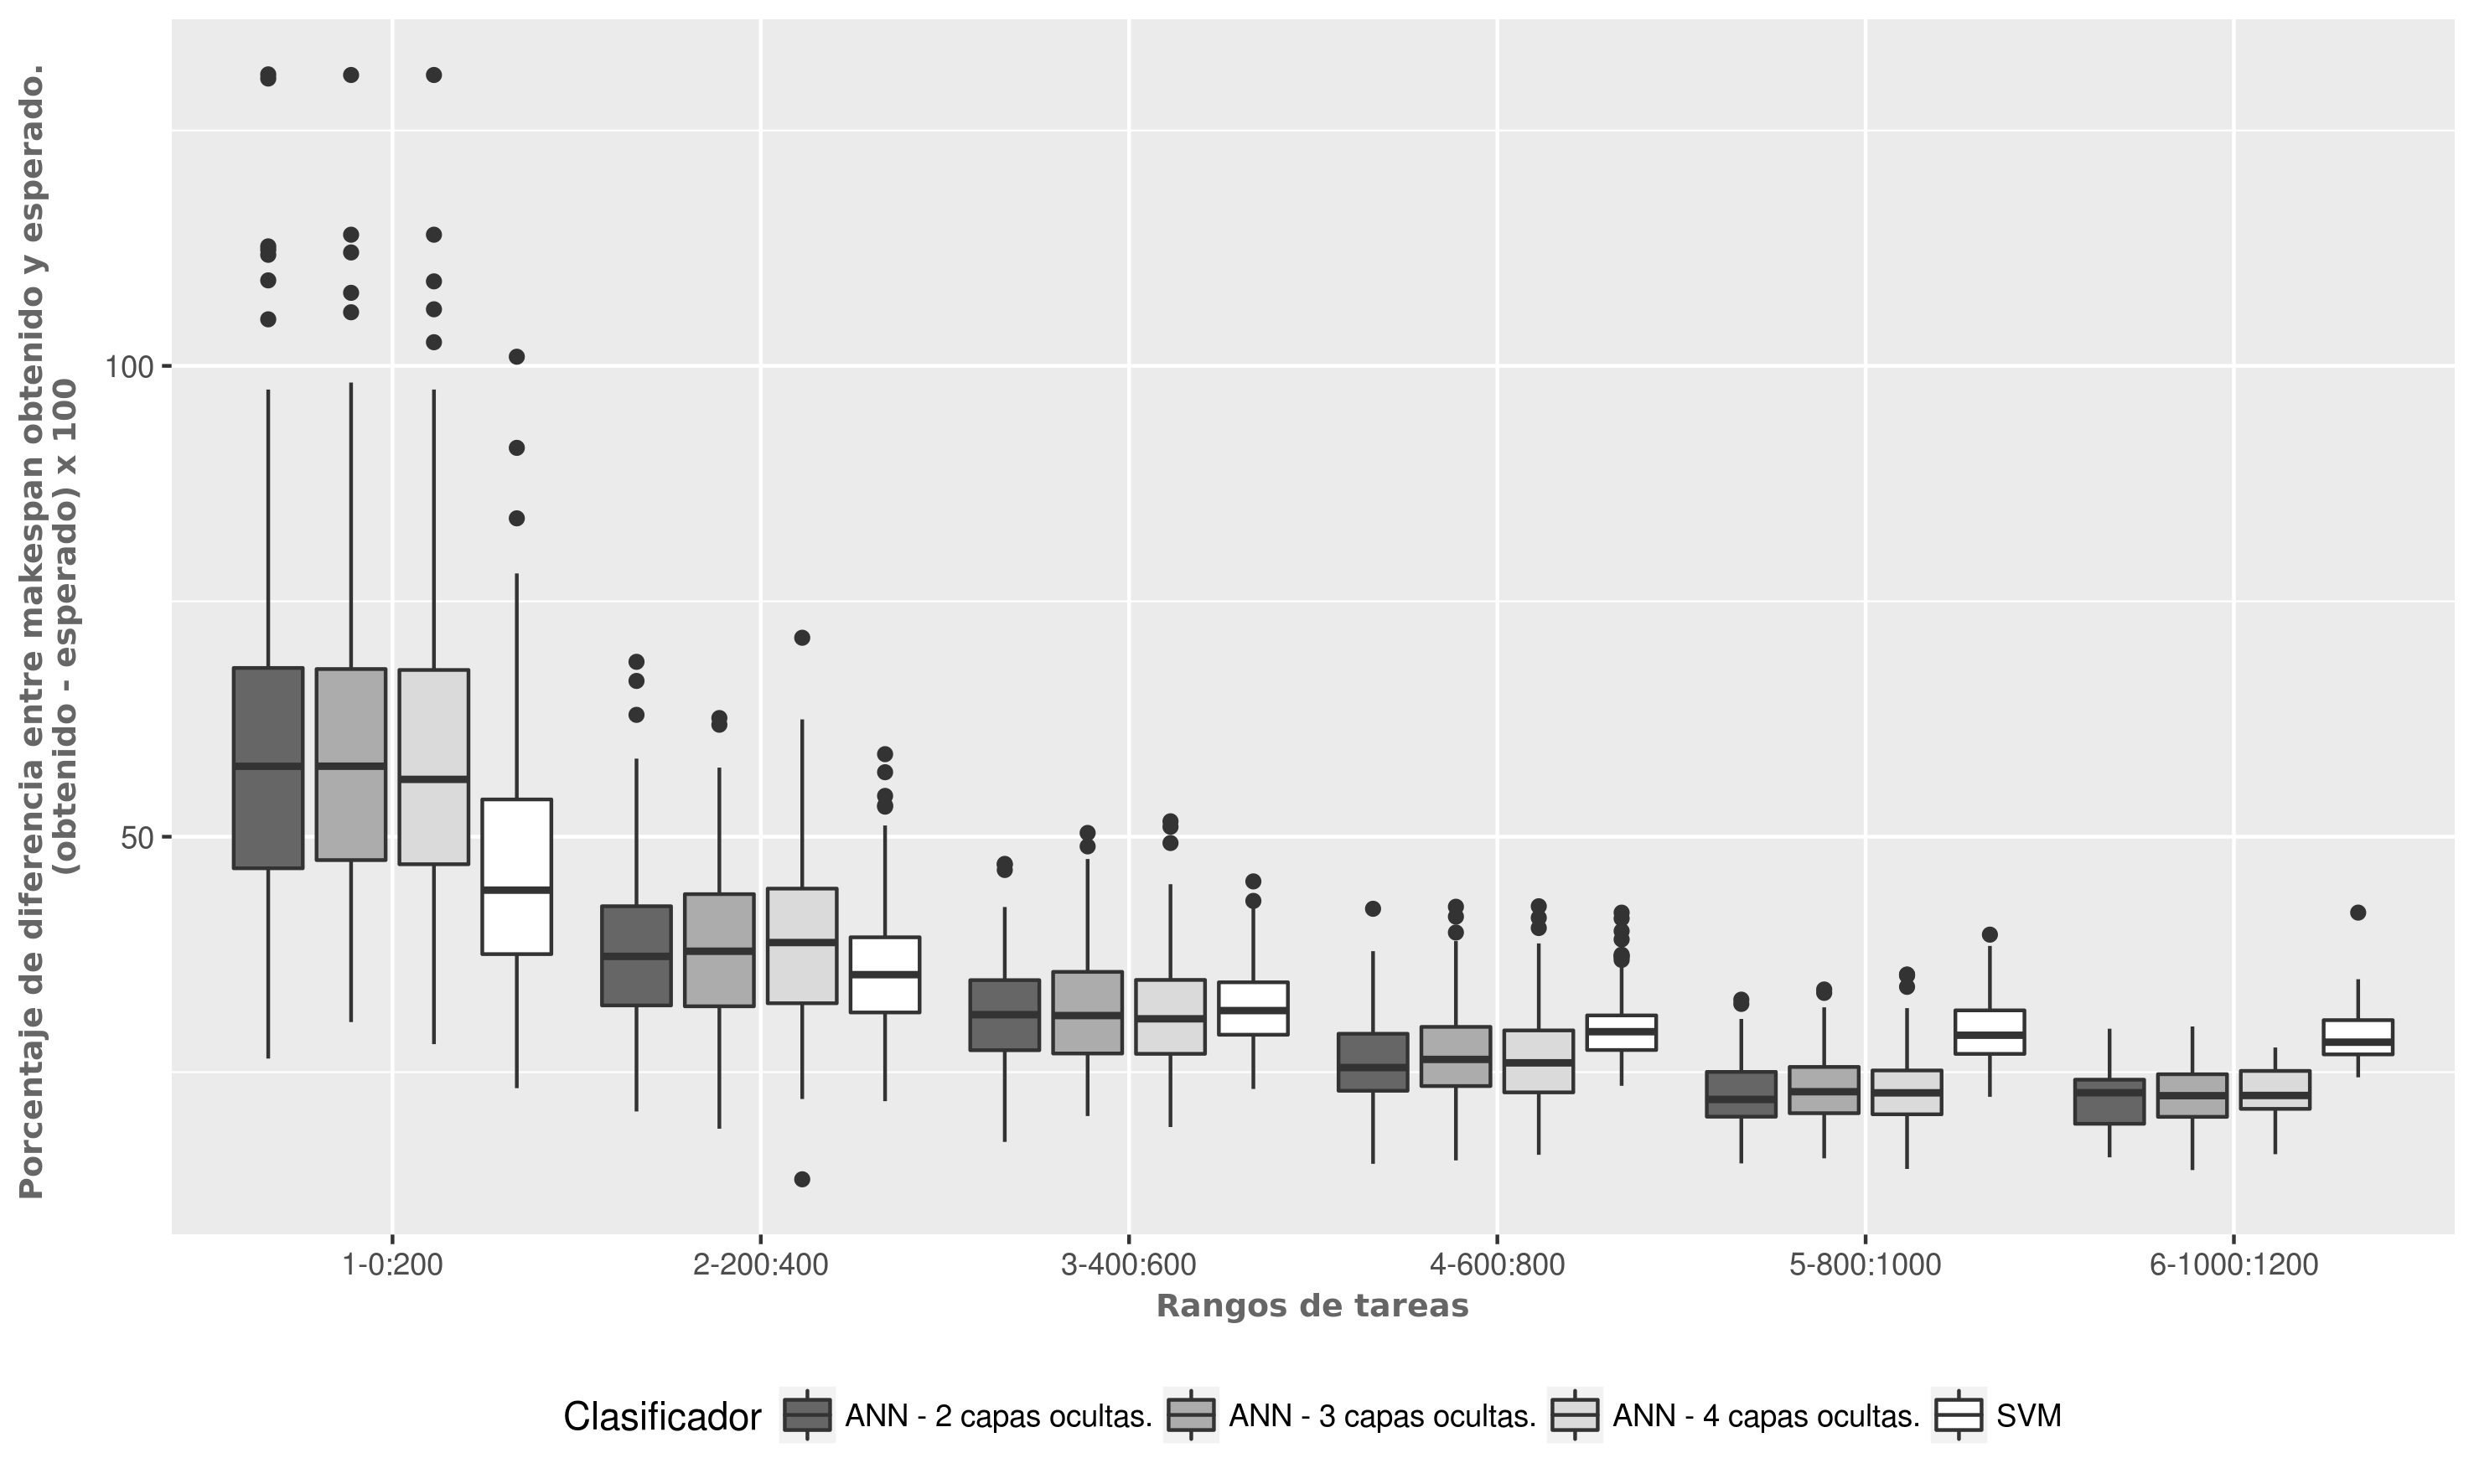
\includegraphics[width=\columnwidth]{imagenes/comparacion_anns_identity.png}
  \caption{Comparación de  la diferencia porcentual  de los resultados de \textit{makespan} para redes neuronales con función de activación \textit{identity}, con respecto al \textit{makespan} obtenido por el algoritmo Min-Min.
Se comparan redes neuronales de 2, 3 y 4 capas.
Así también se muestran los resultados obtenidos con el algoritmo de SVM.}
  \label{fig:identity234}
\end{figure}

\begin{figure}[H]
  \centering
  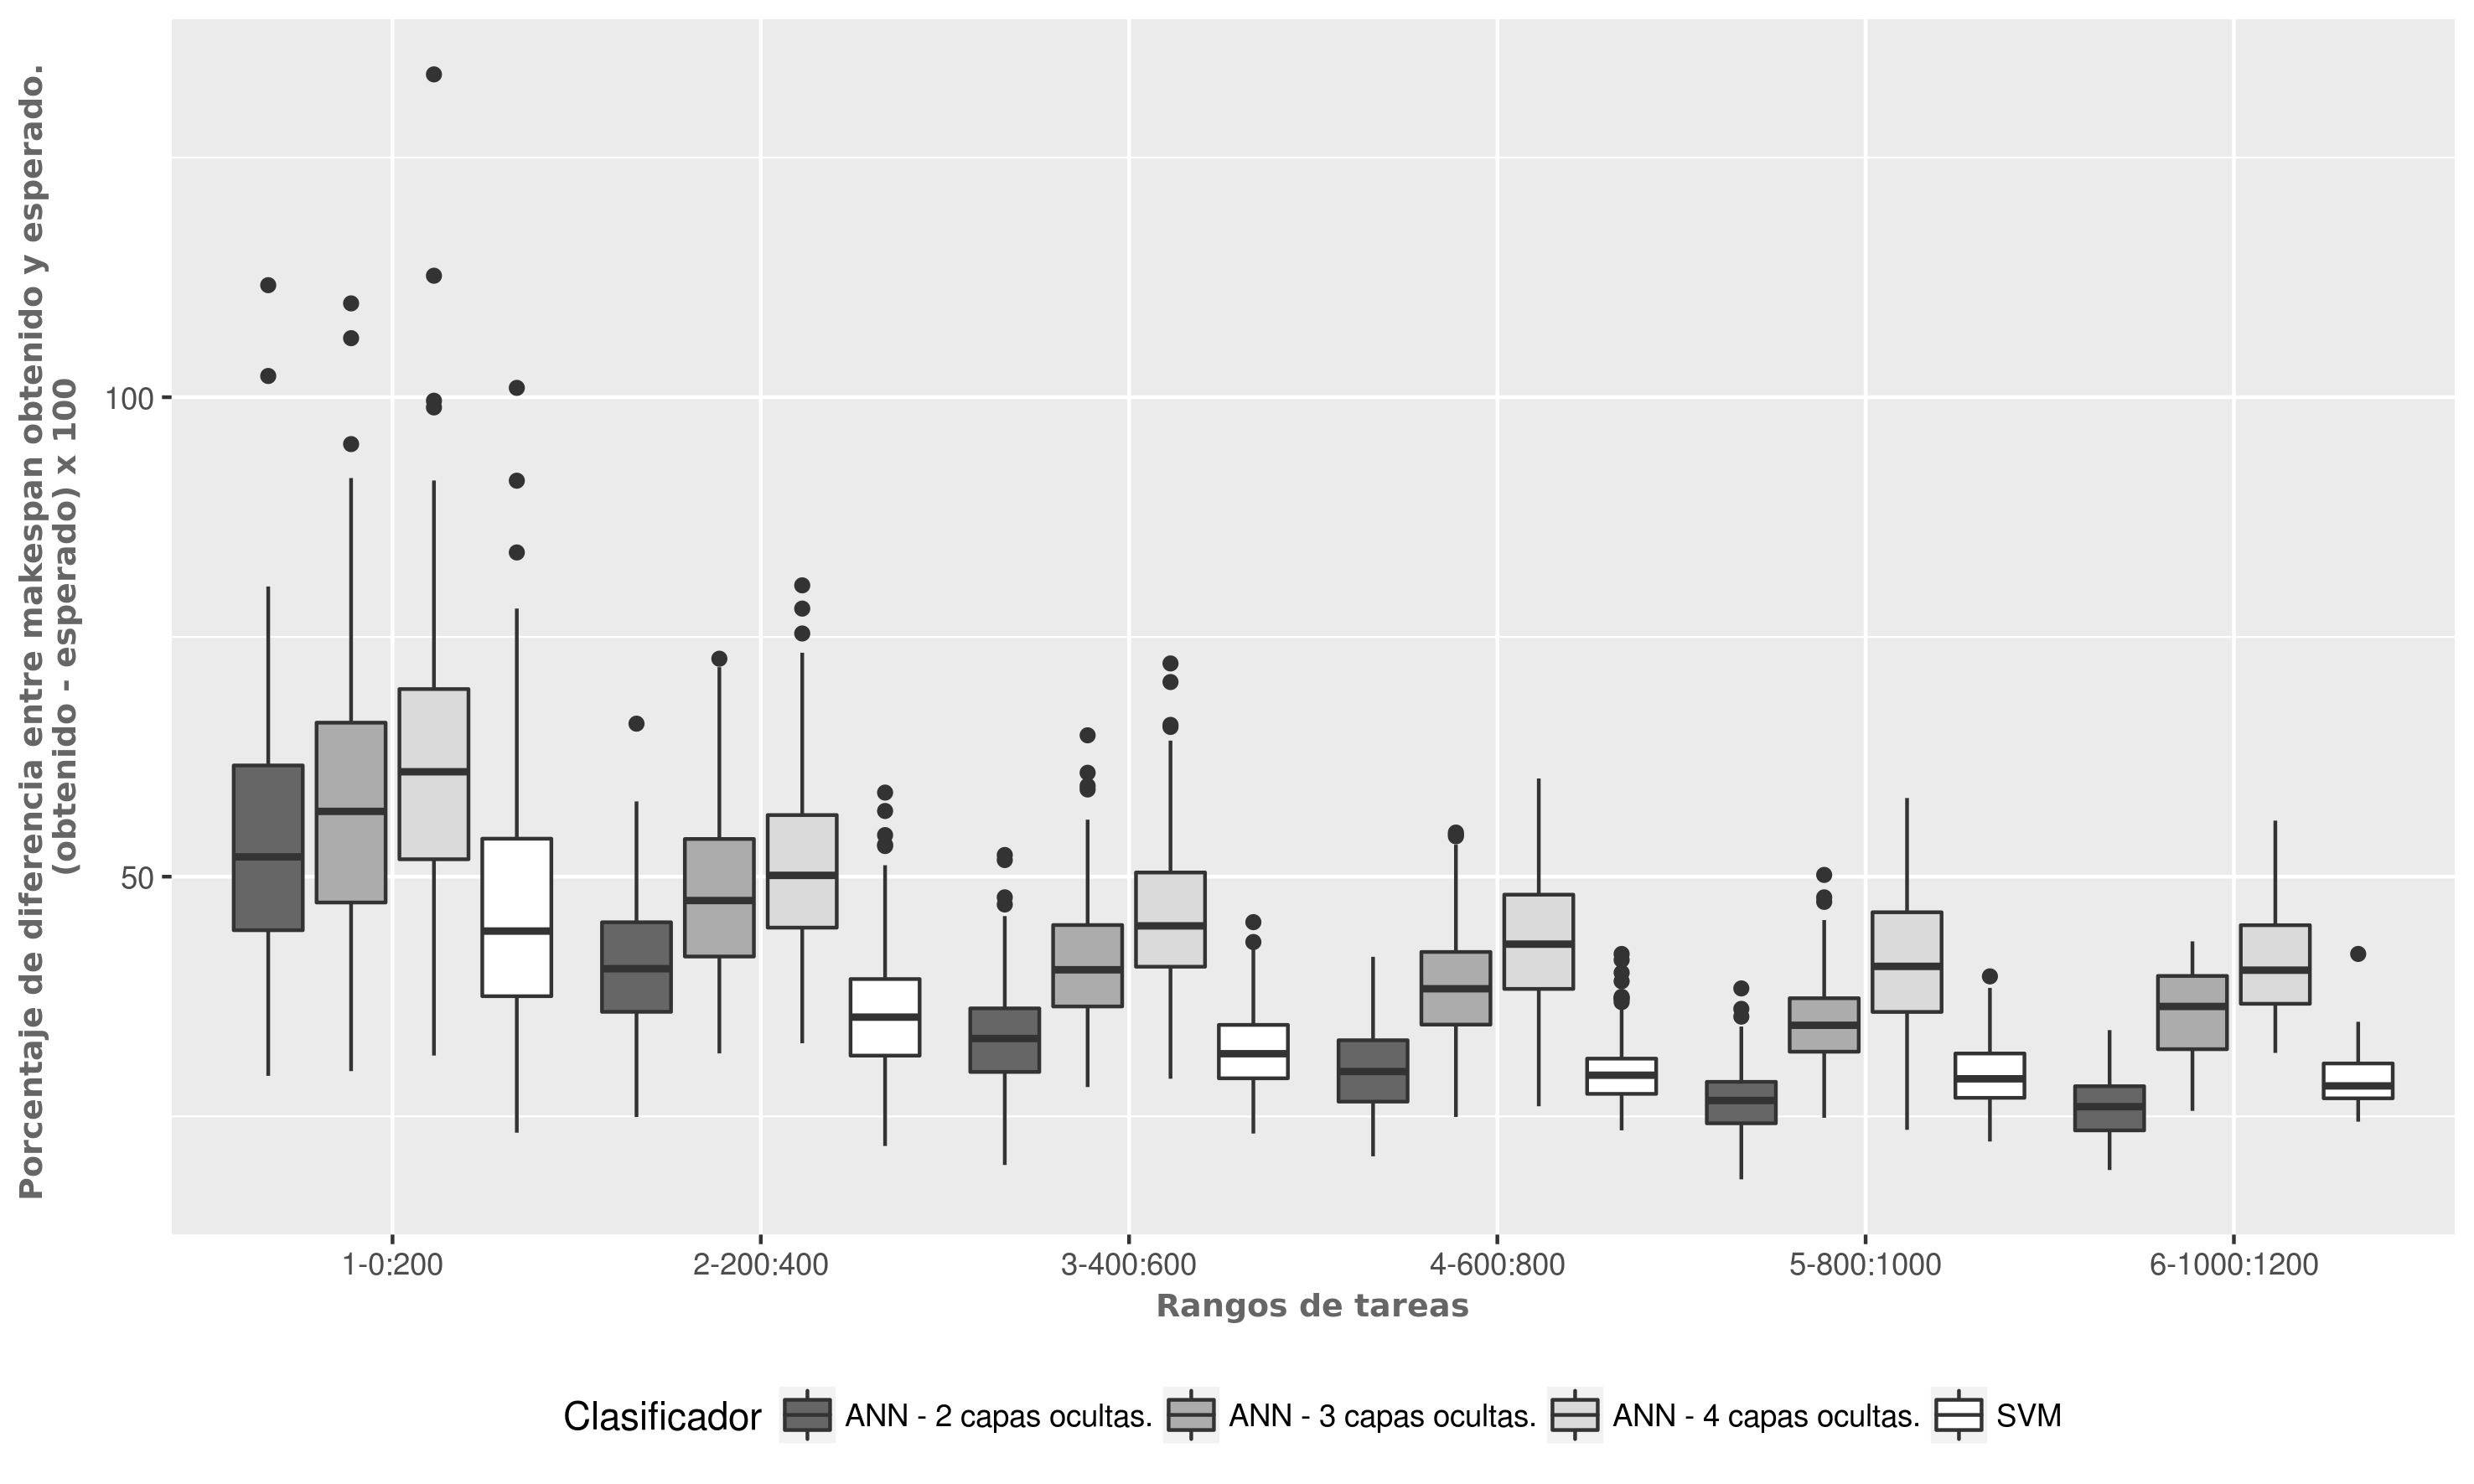
\includegraphics[width=\columnwidth]{imagenes/comparacion_anns_tanh.png}
  \caption{Comparación de  la diferencia porcentual  de los resultados de \textit{makespan} para redes neuronales con función de activación \textit{tanh}, con respecto al \textit{makespan} obtenido por el algoritmo Min-Min.
Se comparan redes neuronales de 2, 3 y 4 capas.
Así también se muestran los resultados obtenidos con el algoritmo de SVM.}
  \label{fig:tanh234}
\end{figure}

\section{Red neuronal con activación \textit{relu} de dos capas ocultas}

La Figura \ref{fig:relu_makespan} muestra con más claridad la diferencia porcentual de \textit{makespan} entre la red neuronal de dos capas ocultas con función de activación \textit{relu} y la SVM con respecto al \textit{makespan} esperado.
Como ya se observó, la SVM muestra valores más próximos a los valores esperados que la red neuronal. 

\paragraph{} Por otro lado, la Figura \ref{fig:relu_accuracy} muestra la precisión de la clasificación para ambos clasificadores.
Se observa que la precisión en clasificación aumenta a medida que la dimensión de las instancias de prueba aumenta, tanto para la red neuronal como para la SVM. 

\begin{figure}[H]
  \centering
  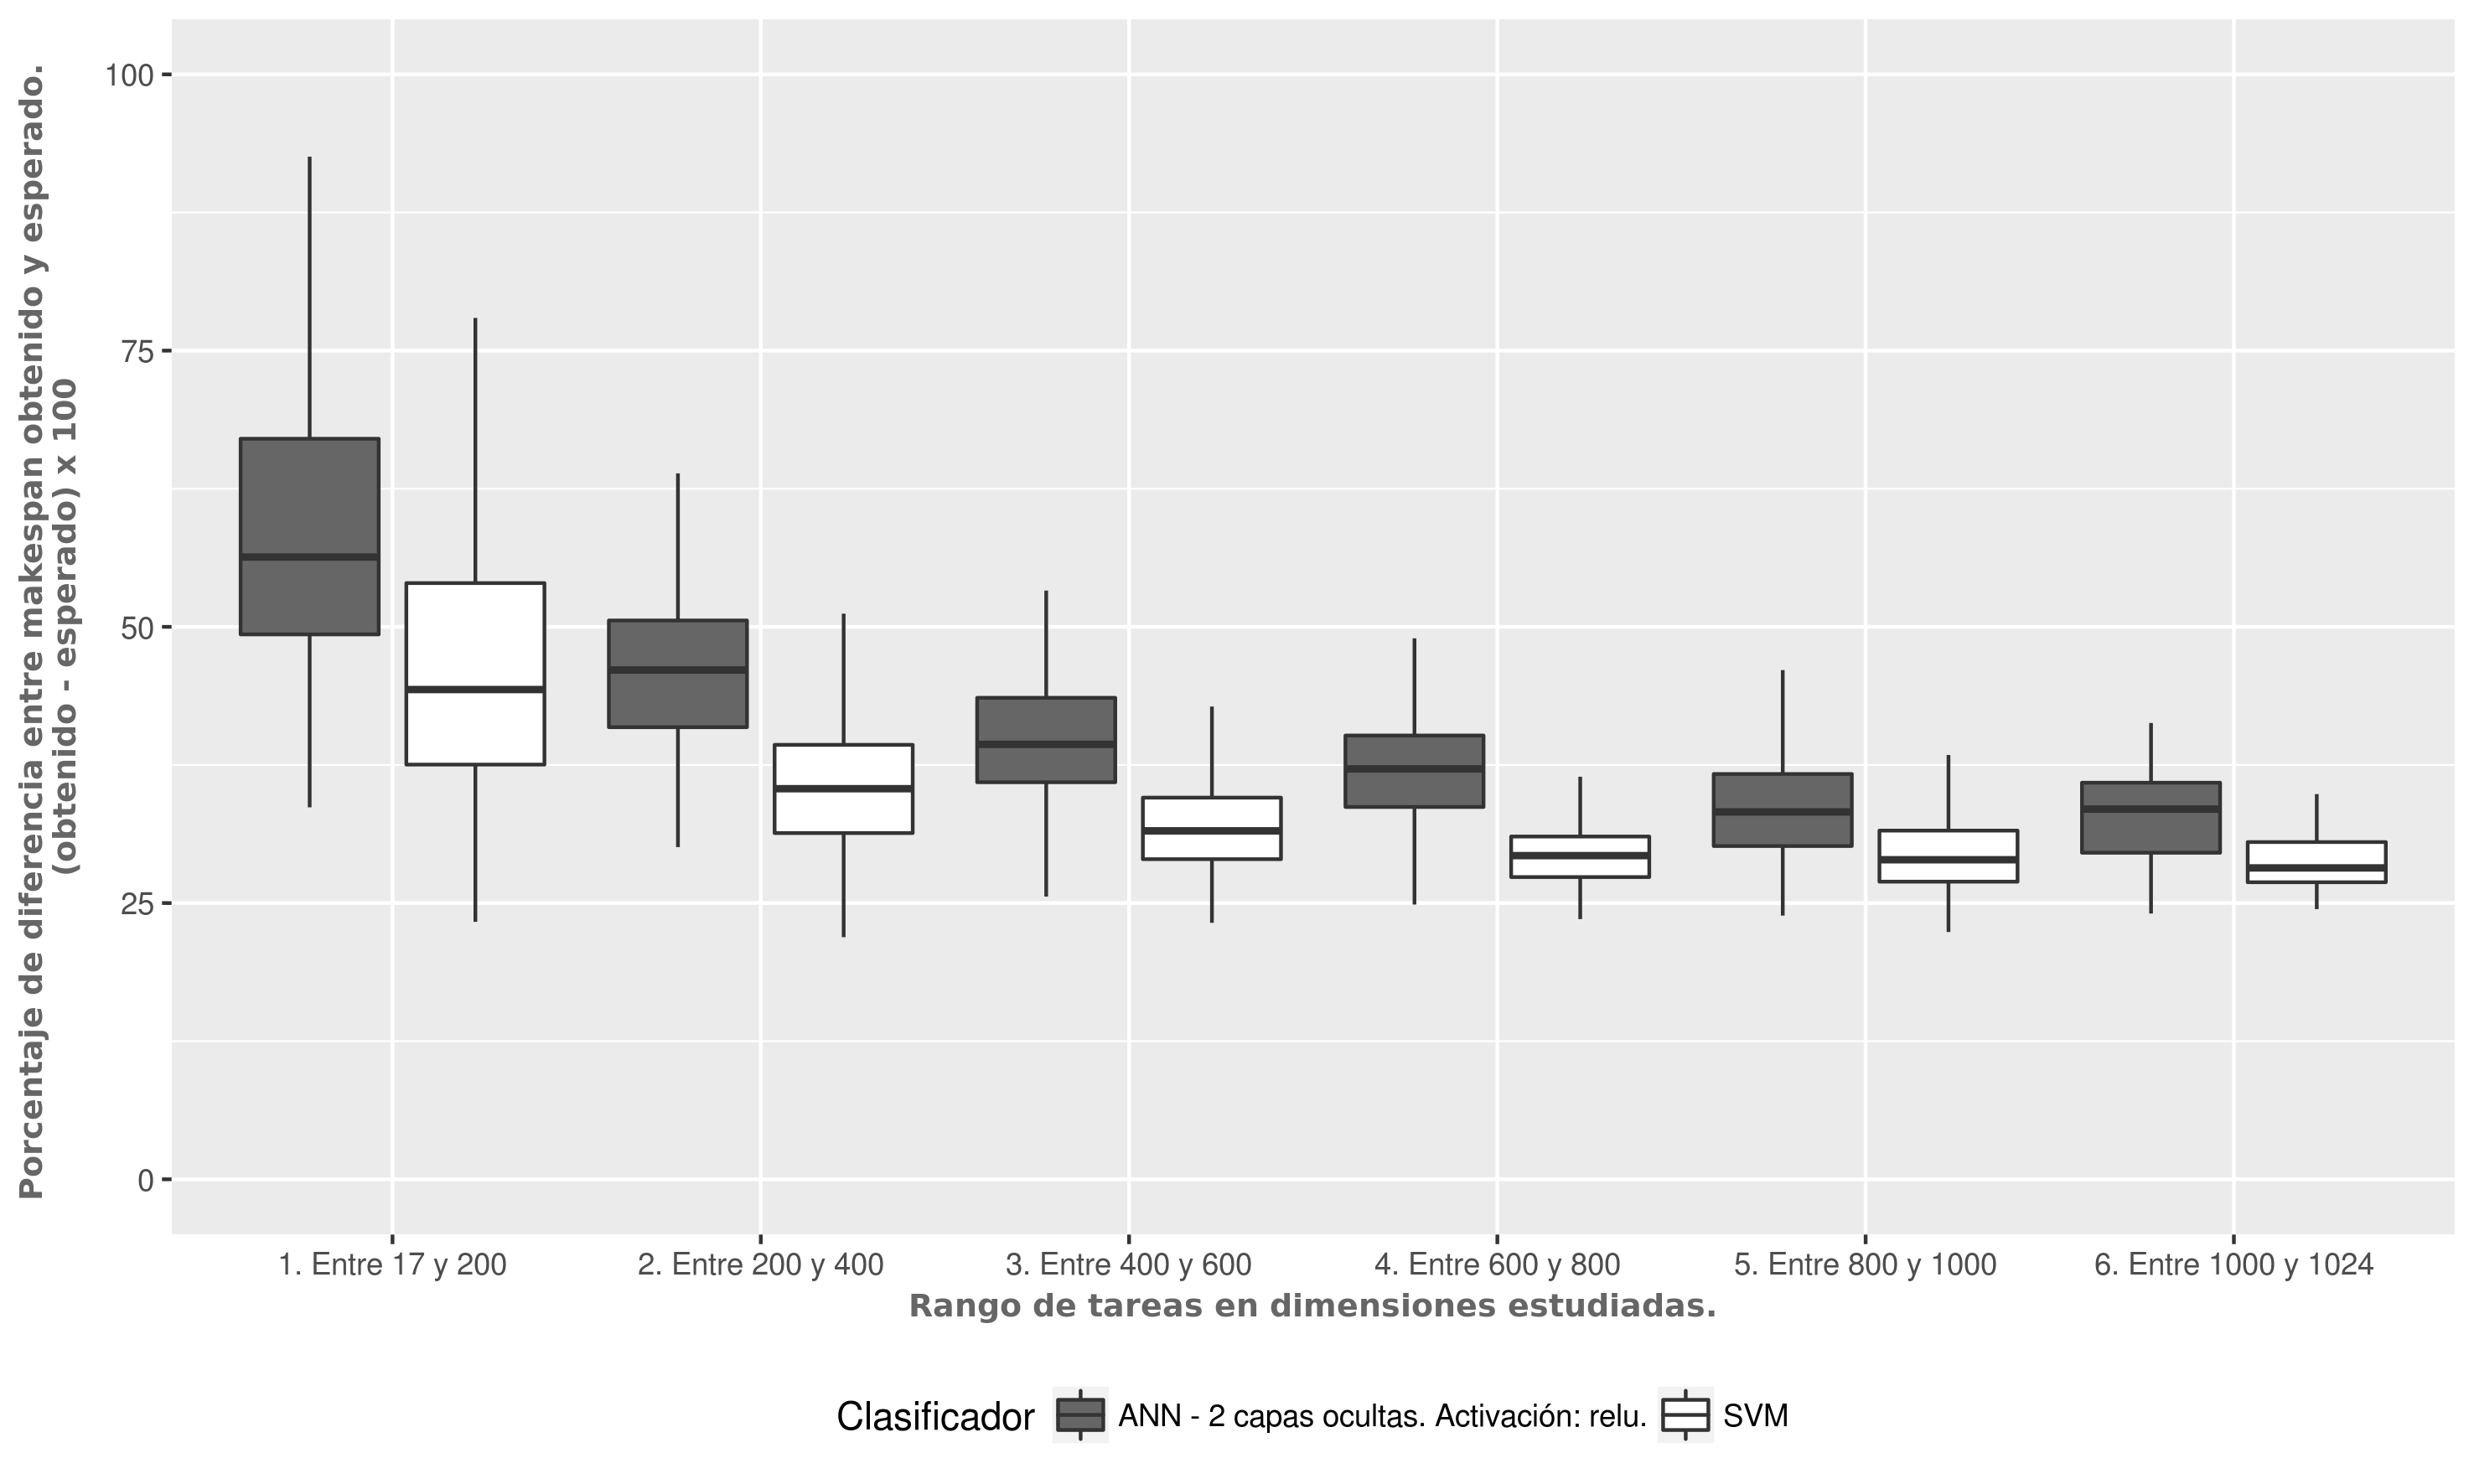
\includegraphics[width=\columnwidth]{imagenes/relu/2_medianas_diferenciasann_2_capas_ocultas_relu.png}
  \caption{Comparación de la diferencia porcentual de \textit{makespan} para la red neuronal con activación \textit{relu}, de dos capas ocultas con respecto a los valores esperados obtenidos con el algoritmo Min-Min.
Así también se muestran los resultados obtenidos para la SVM.
Los resultados se muestran divididos en rangos de dimensión desde $ 17 \times 16$ a $ 1024 \times 16$.}
  \label{fig:relu_makespan}
\end{figure}

\paragraph{}La precisión de la red neuronal es levemente mayor que la precisión de la SVM.
Esto, en comparación con la diferencia de \textit{makespan} de la Figura \ref{fig:relu_makespan}, es de interés, dado que si bien la precisión de la red neuronal es levemente mejor, la SVM genera mejores resultados en términos de \textit{makespan}.
Este escenario también fue identificado para las demás redes neuronales en las cuales se profundizaron los estudios. 

\paragraph{} Para poder explicar lo antedicho, fue calculado el porcentaje de selección de mejores máquinas para ambos clasificadores, como se menciona en la sección dedicada a la implementación.
La Figura \ref{fig:relu_maquinas_mejores} muestra dicha métrica para ambos clasificadores.
En esta se observa que la SVM elige más máquinas con menor tiempo de ejecución que la red neuronal, cuando  se seleccionan máquinas diferentes a las esperadas. 

\begin{figure}[H]
  \centering
  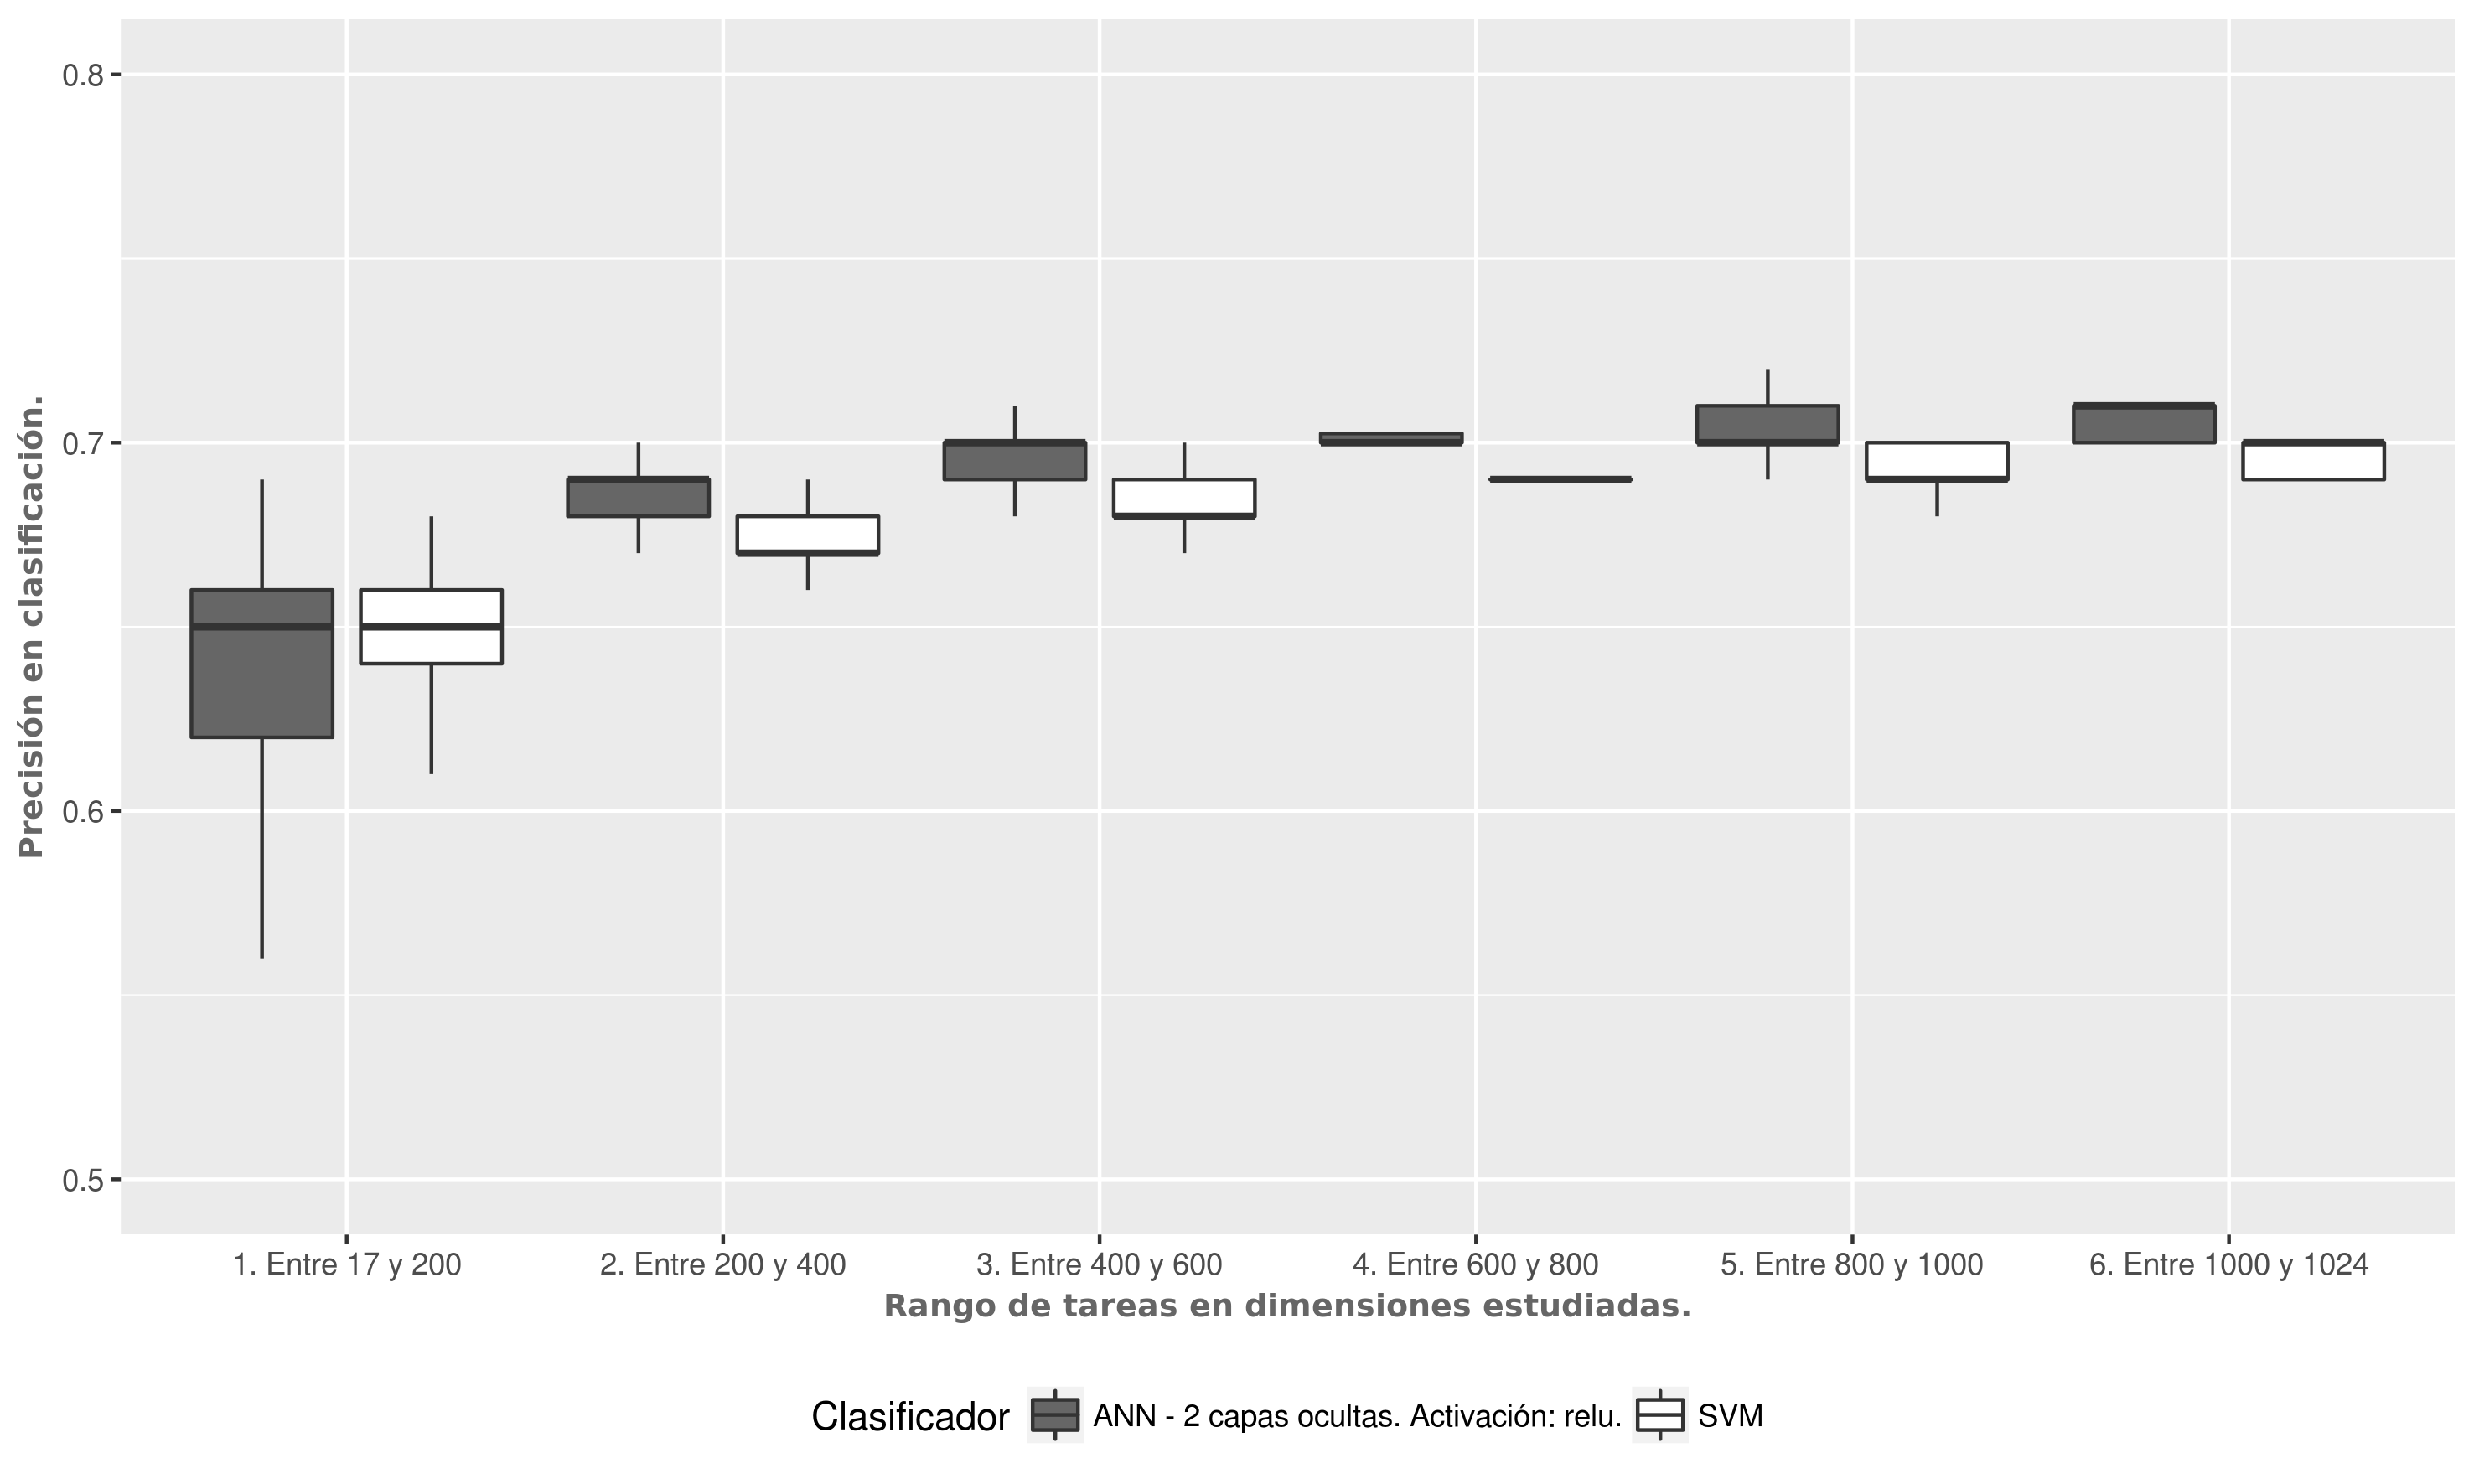
\includegraphics[width=\columnwidth]{imagenes/relu/3_accuracy_ann_2_capas_ocultas_relu.png}
  \caption{Precisión en clasificación para la red neuronal con función de activación \textit{relu} de dos capas ocultas y para la SVM.
Los resultados se muestran divididos en rangos de dimensión desde $ 17 \times 16$ a $ 1024 \times 16$.}
  \label{fig:relu_accuracy}
\end{figure}

\begin{figure}[H]
  \centering
  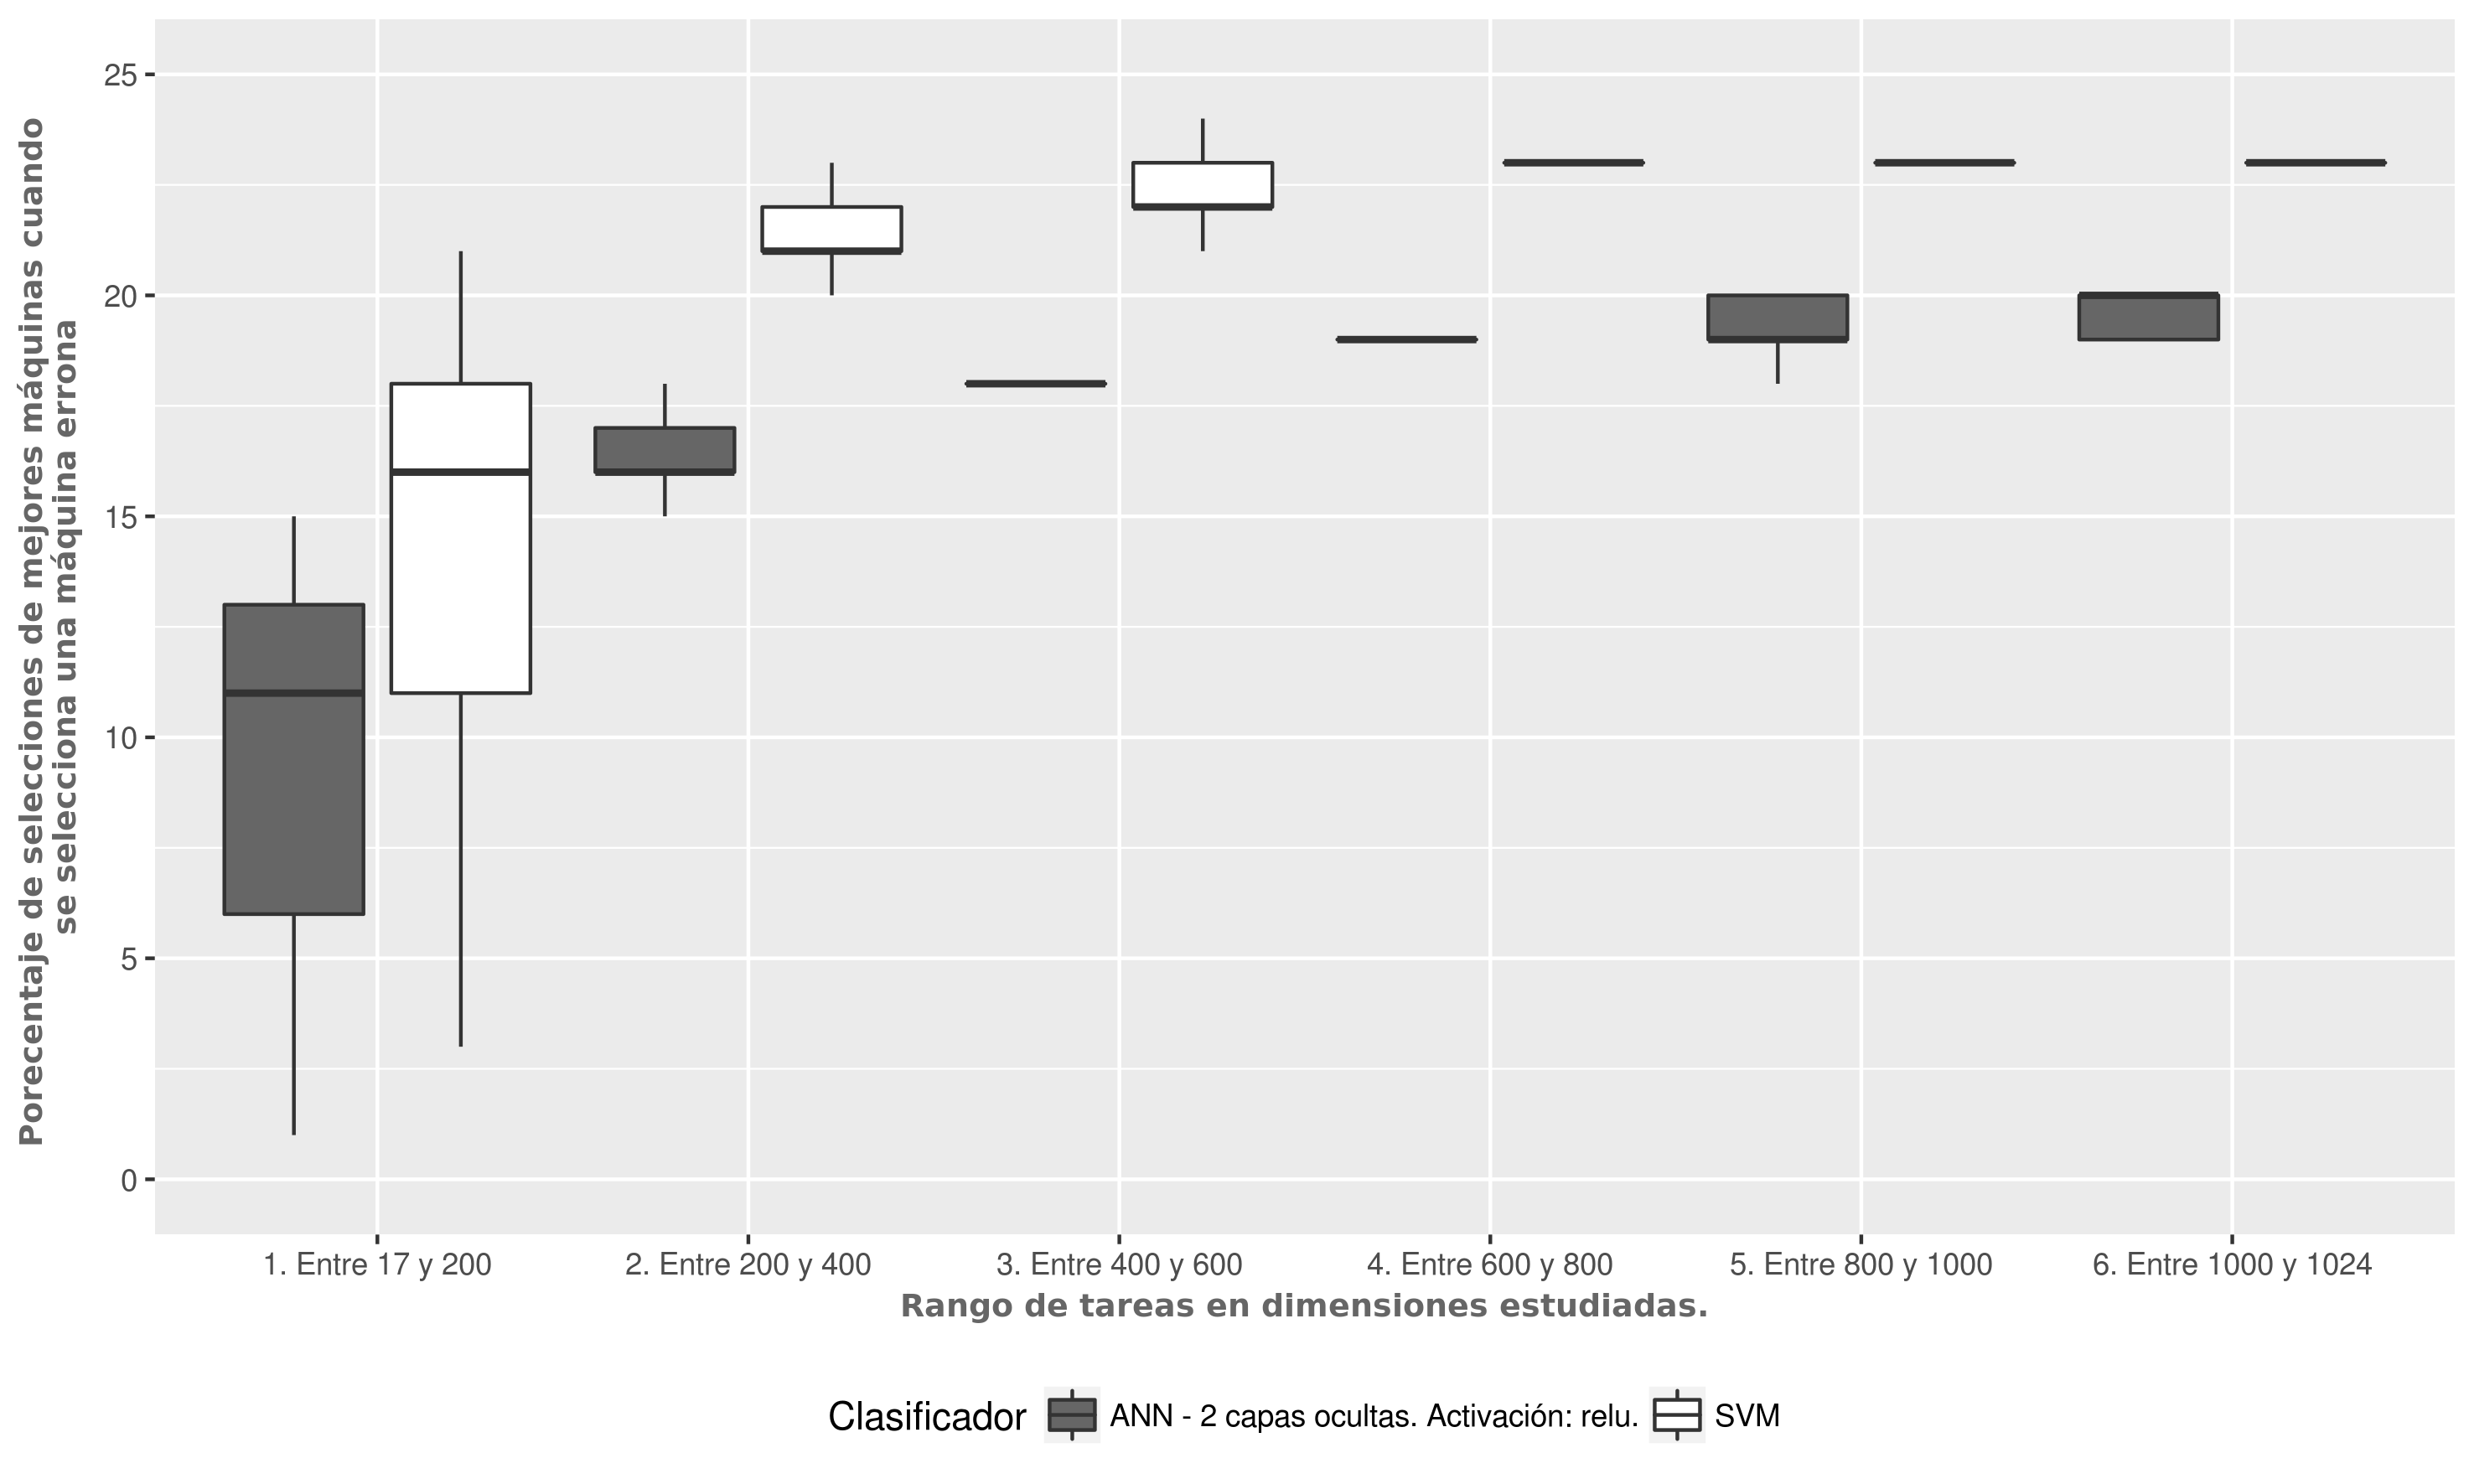
\includegraphics[width=\columnwidth]{imagenes/relu/4_porcentaje_maquinas_mejores_ann_2_capas_ocultas_relu.png}
  \caption{Porcentaje de selección de máquinas mejores frente a una selección diferente a la esperada para la red neuronal con activación \textit{relu} de dos capas ocultas y para la SVM.}
  \label{fig:relu_maquinas_mejores}
\end{figure}
 
\section{Red neuronal con activación \textit{identity} de dos capas ocultas}

La Figura \ref{fig:identity_makespan} muestra la diferencia porcentual de \textit{makespan} para la red neuronal con función de activación \textit{identity} y la SVM, con respecto a los resultados esperados obtenidos con el algoritmo Min-Min.
Se observa que para dimensiones mayores a $ 400 \times 16$, la red neuronal conduce a levemente mejores valores de \textit{makespan} que la SVM.
En este caso, la precisión en la clasificación, que se observa en la Figura \ref{fig:identity_accuracy}, no tiene diferencias sustanciales. 

\begin{figure}[H]
  \centering
  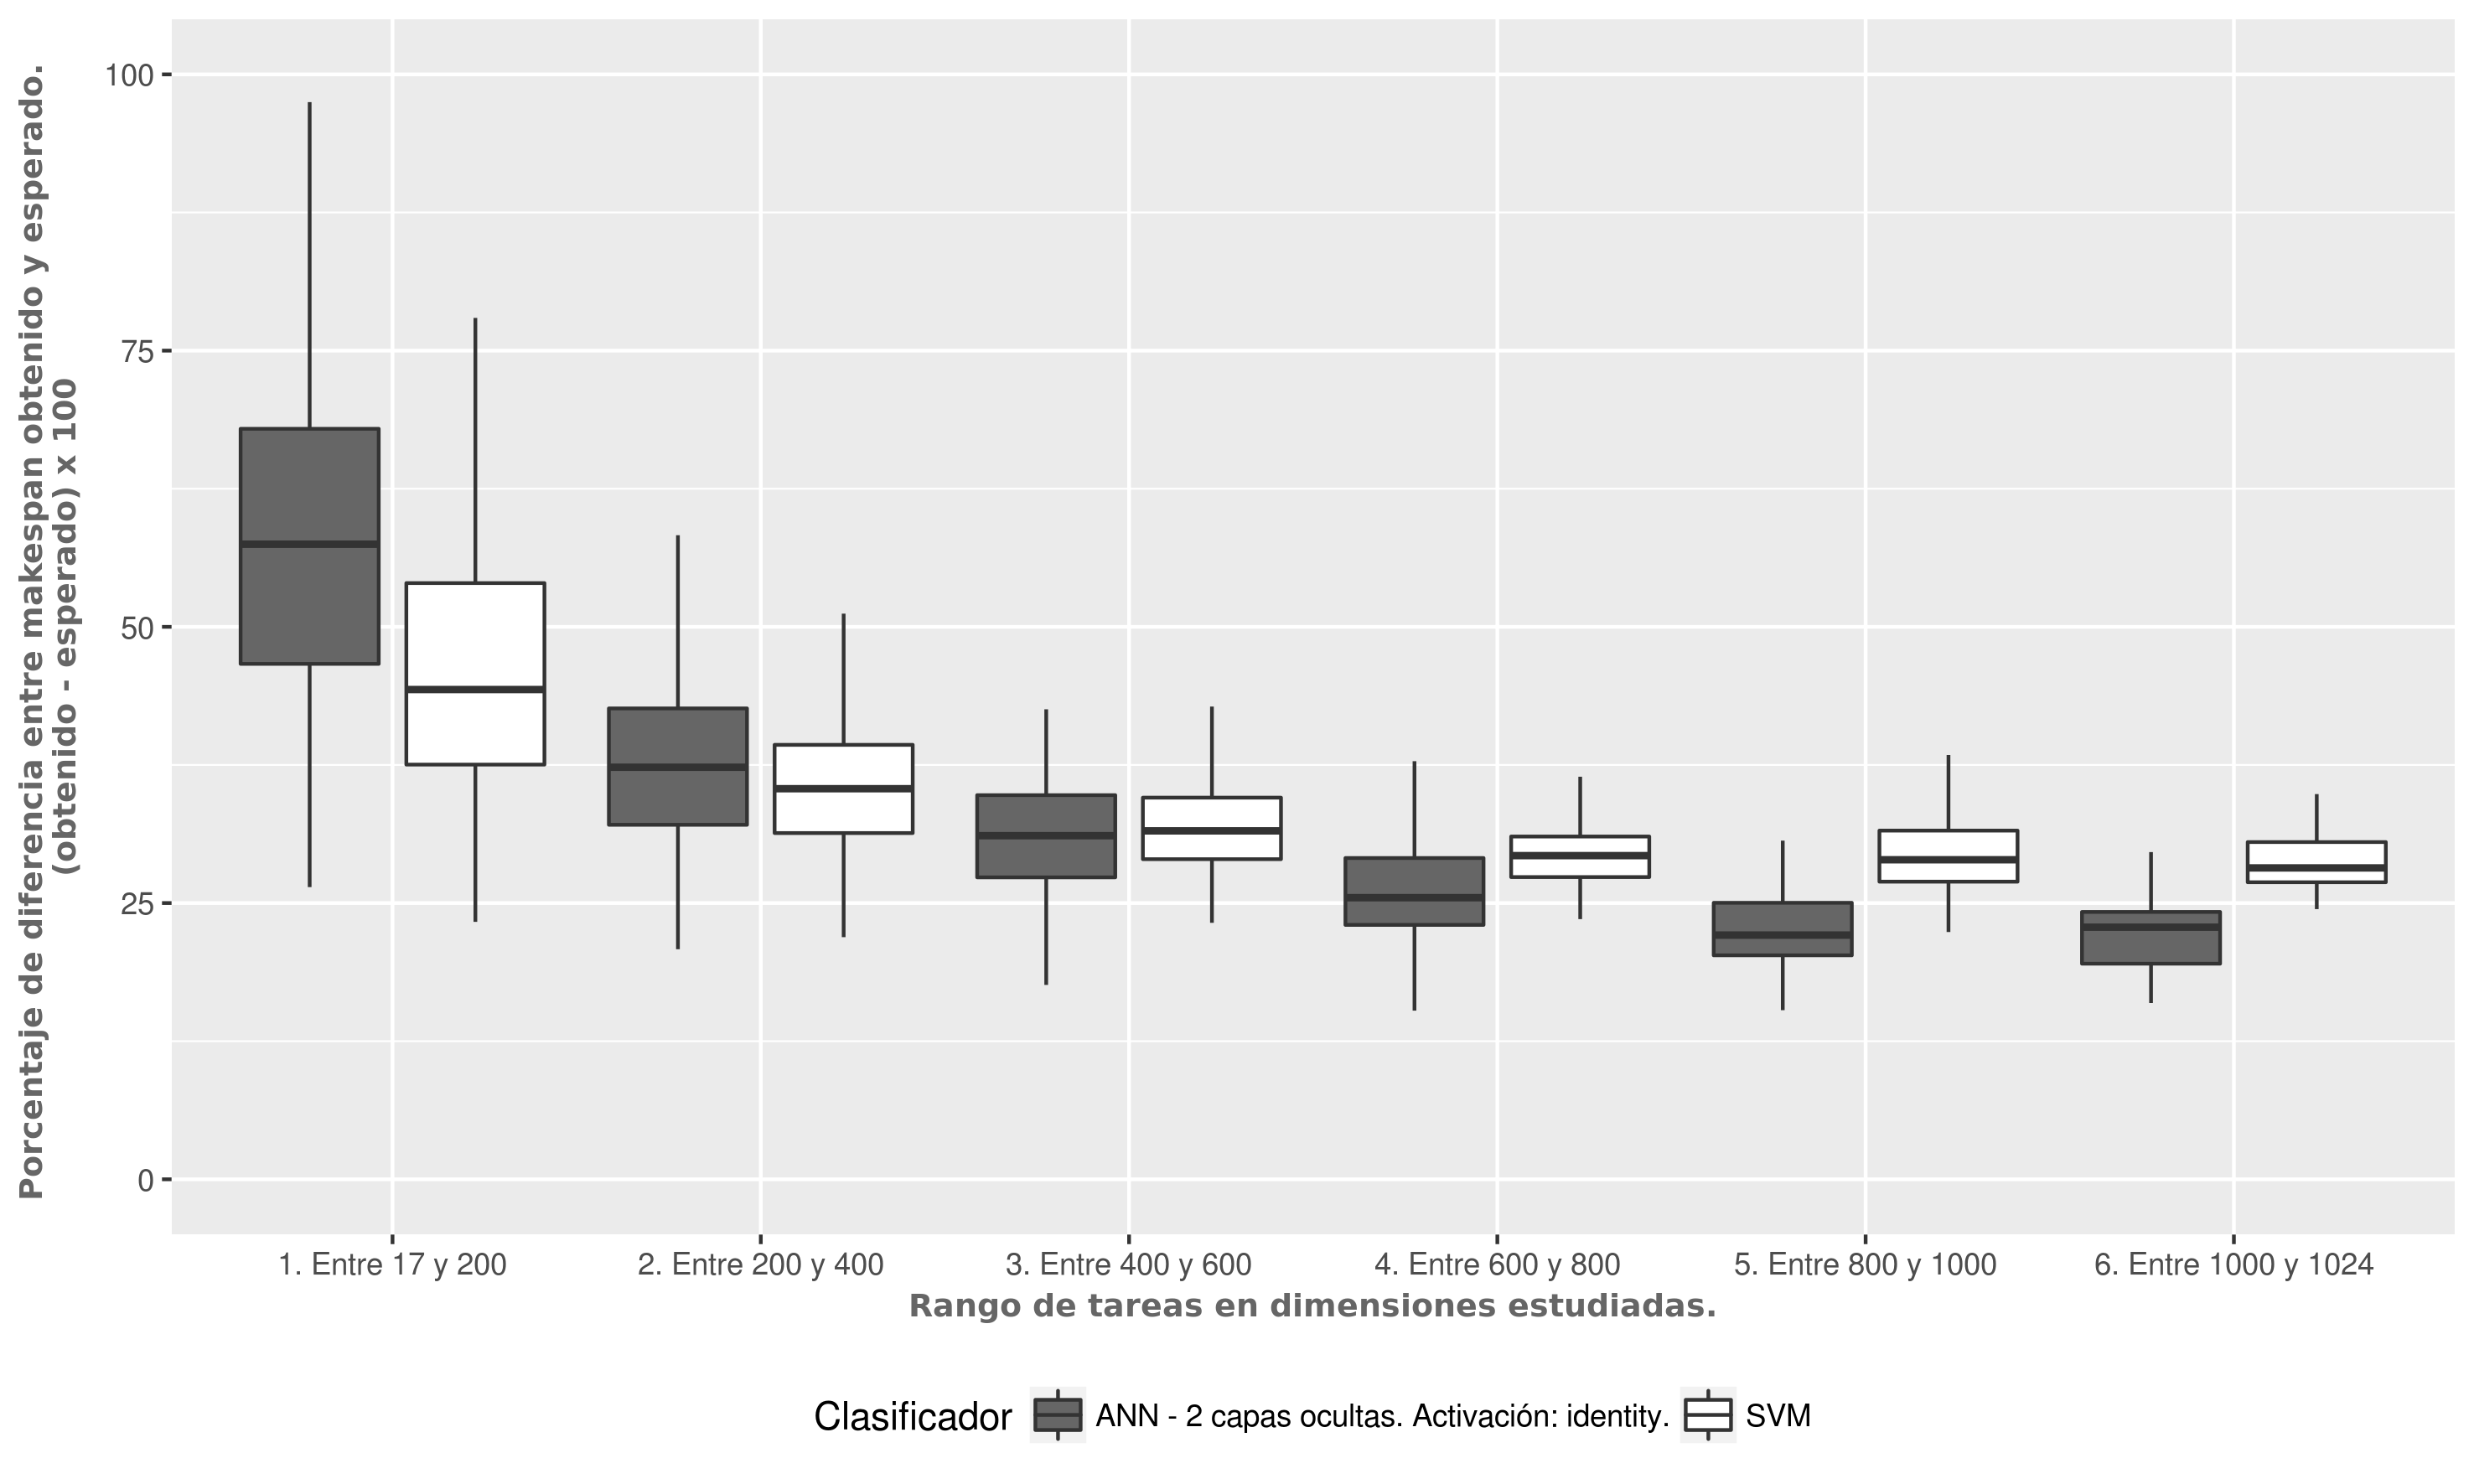
\includegraphics[width=\columnwidth]{imagenes/identity/2_medianas_diferenciasann_2_capas_ocultas_identity.png}
  \caption{Comparación de la diferencia porcentual de \textit{makespan} para la red neuronal con activación \textit{identity}, de dos capas ocultas con respecto a los valores esperados obtenidos con el algoritmo Min-Min.
Así también se muestran los resultados obtenidos para la SVM.
Los resultados se muestran divididos en rangos de dimensión desde $ 17 \times 16$ a $ 1024 \times 16$}
  \label{fig:identity_makespan}
\end{figure}

\begin{figure}[H]
  \centering
  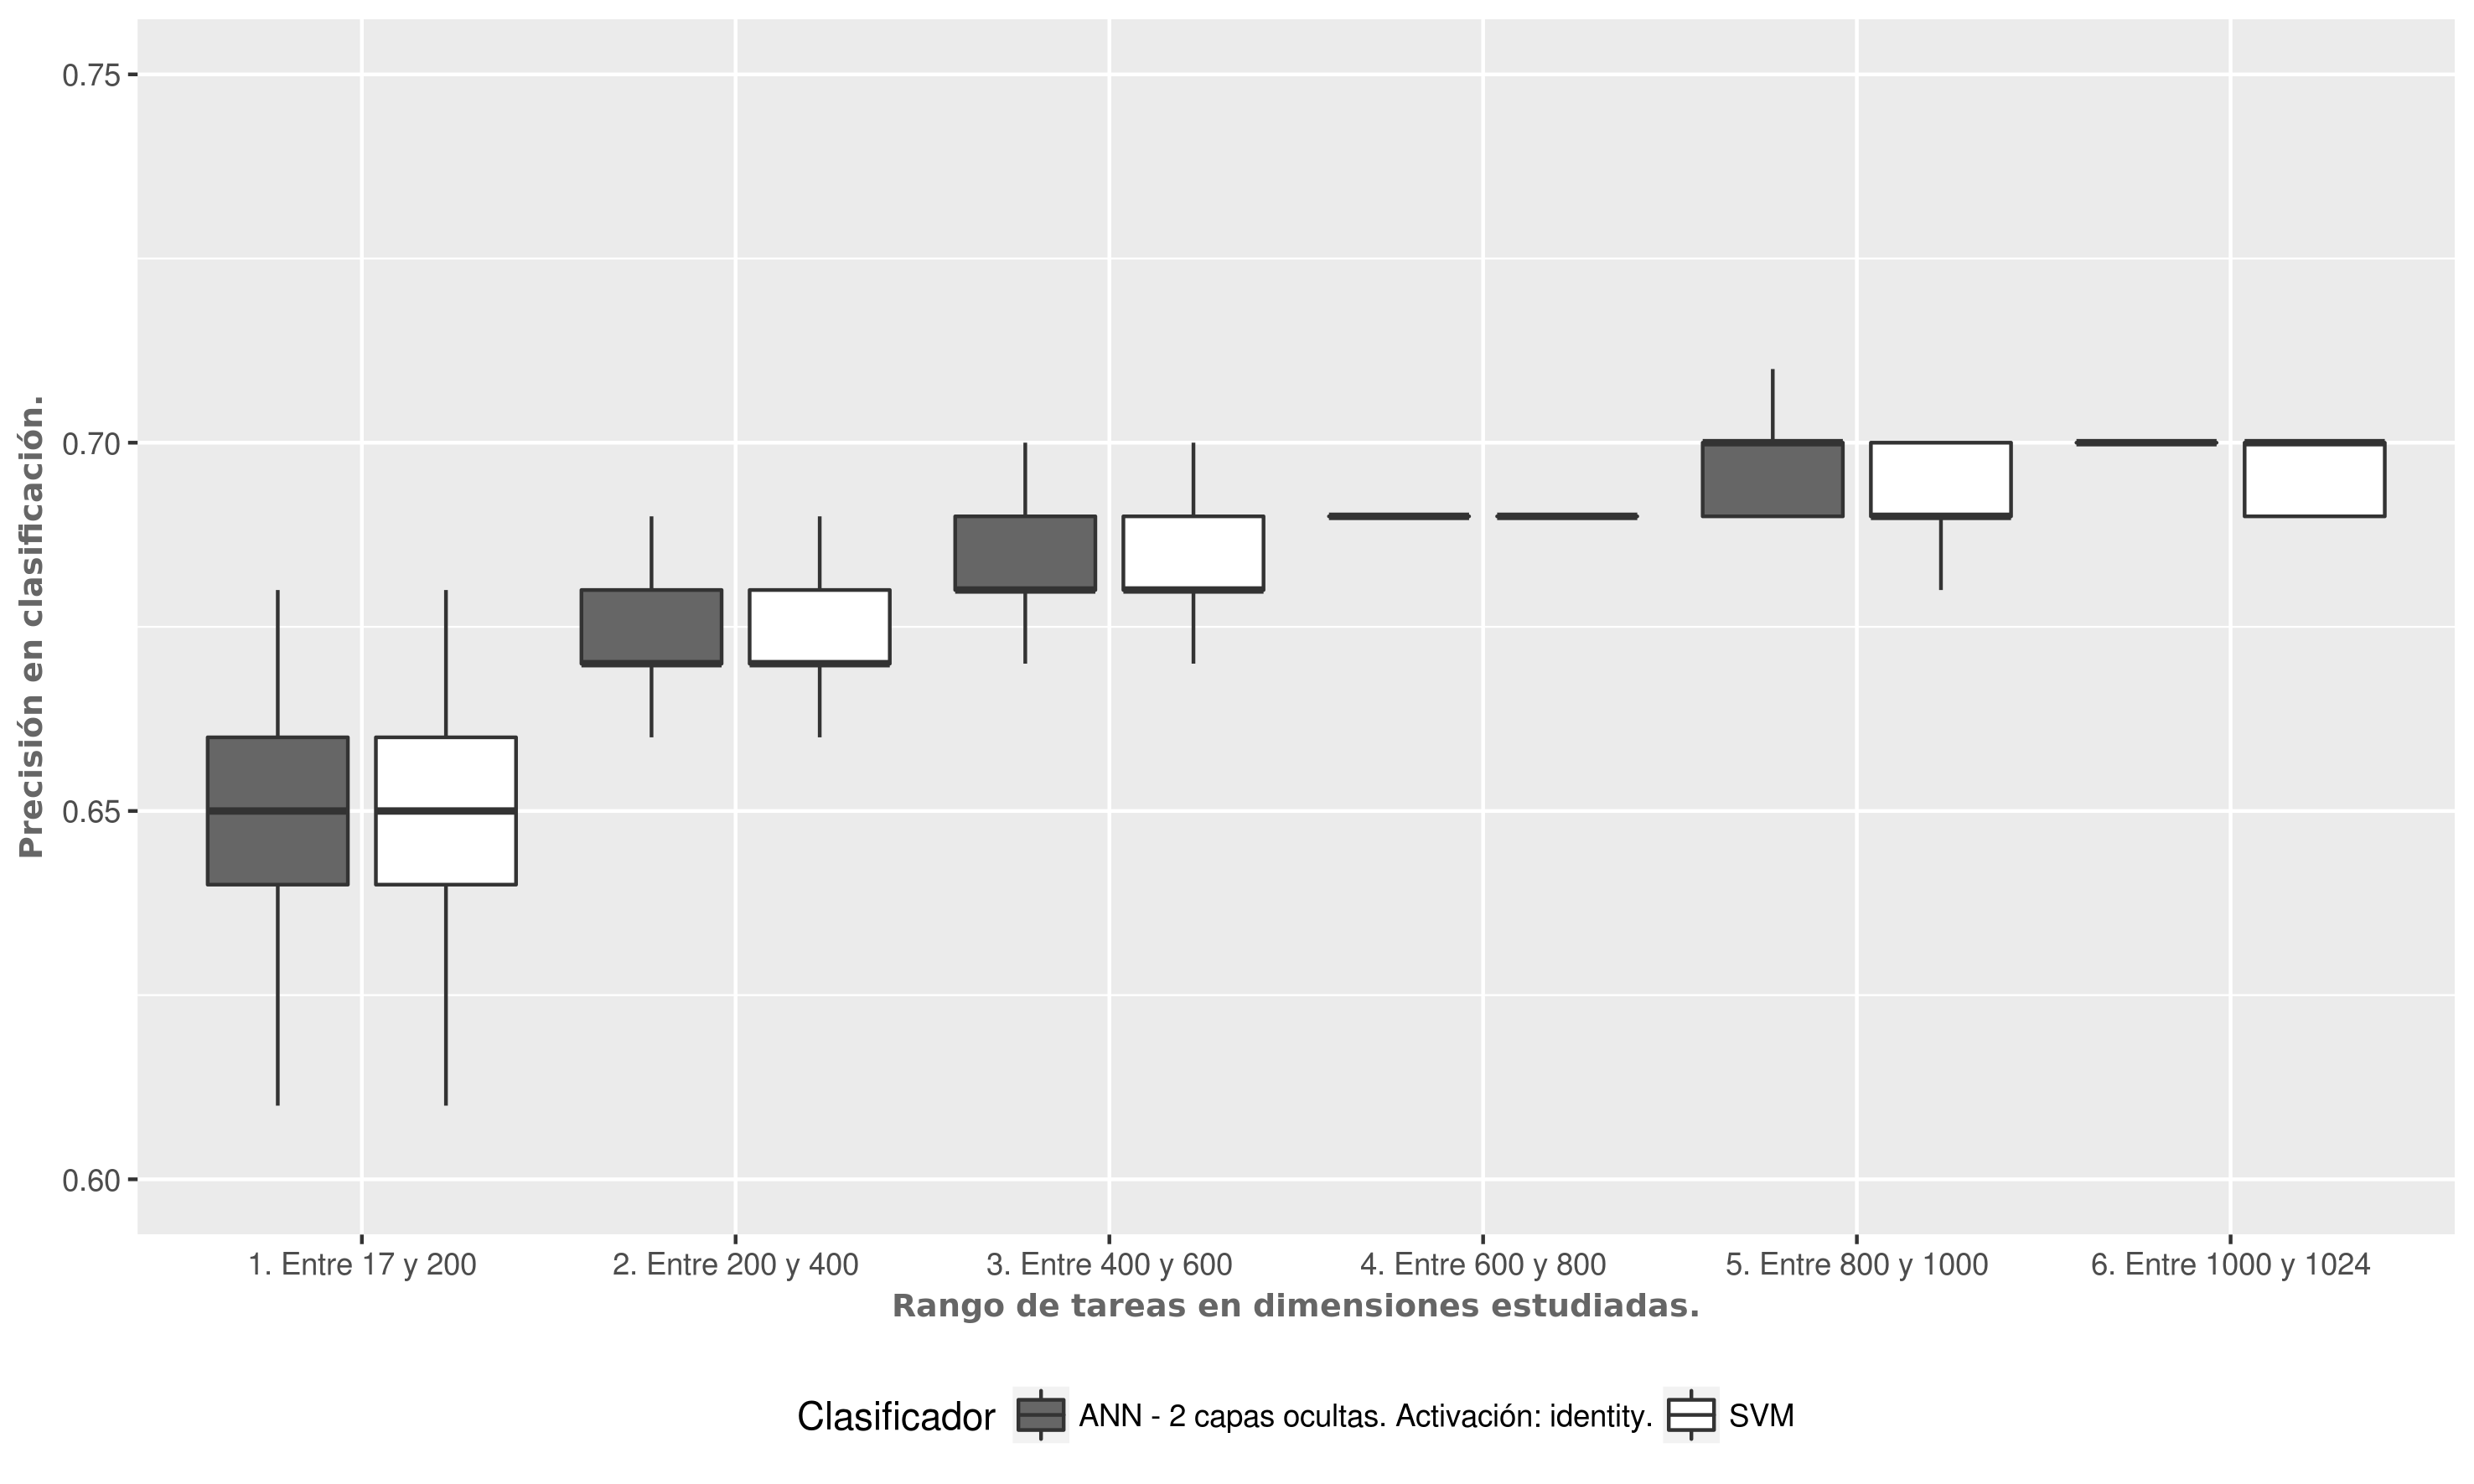
\includegraphics[width=\columnwidth]{imagenes/identity/3_accuracy_ann_2_capas_ocultas_identity.png}
  \caption{Precisión en clasificación para la red neuronal con función de activación \textit{identity} y para la SVM.
Los resultados se muestran divididos en rangos de dimensión desde $ 17 \times 16$ a $ 1024 \times 16$.}
  \label{fig:identity_accuracy}
\end{figure}

\paragraph{}Al observar el porcentaje de mejores máquinas seleccionadas frente a un error en la Figura \ref{fig:identity_mejores}, se observa que la red neuronal selecciona máquinas más rápidas en proporciones similares a la SVM, a diferencia de los resultados presentados para la red neuronal con función de activación \textit{relu}, donde la red neuronal tiende a elegir máquinas más lentas que la SVM frente a un error.
Estos resultados llevan a pensar que el hecho de que la proporción de selección de mejores máquinas por parte de la red neuronal con función de activación \textit{identity} sea mayor que para el caso de \textit{relu}, conduce a una leve disminución del \textit{makespan}. 

\begin{figure}[H]
  \centering
  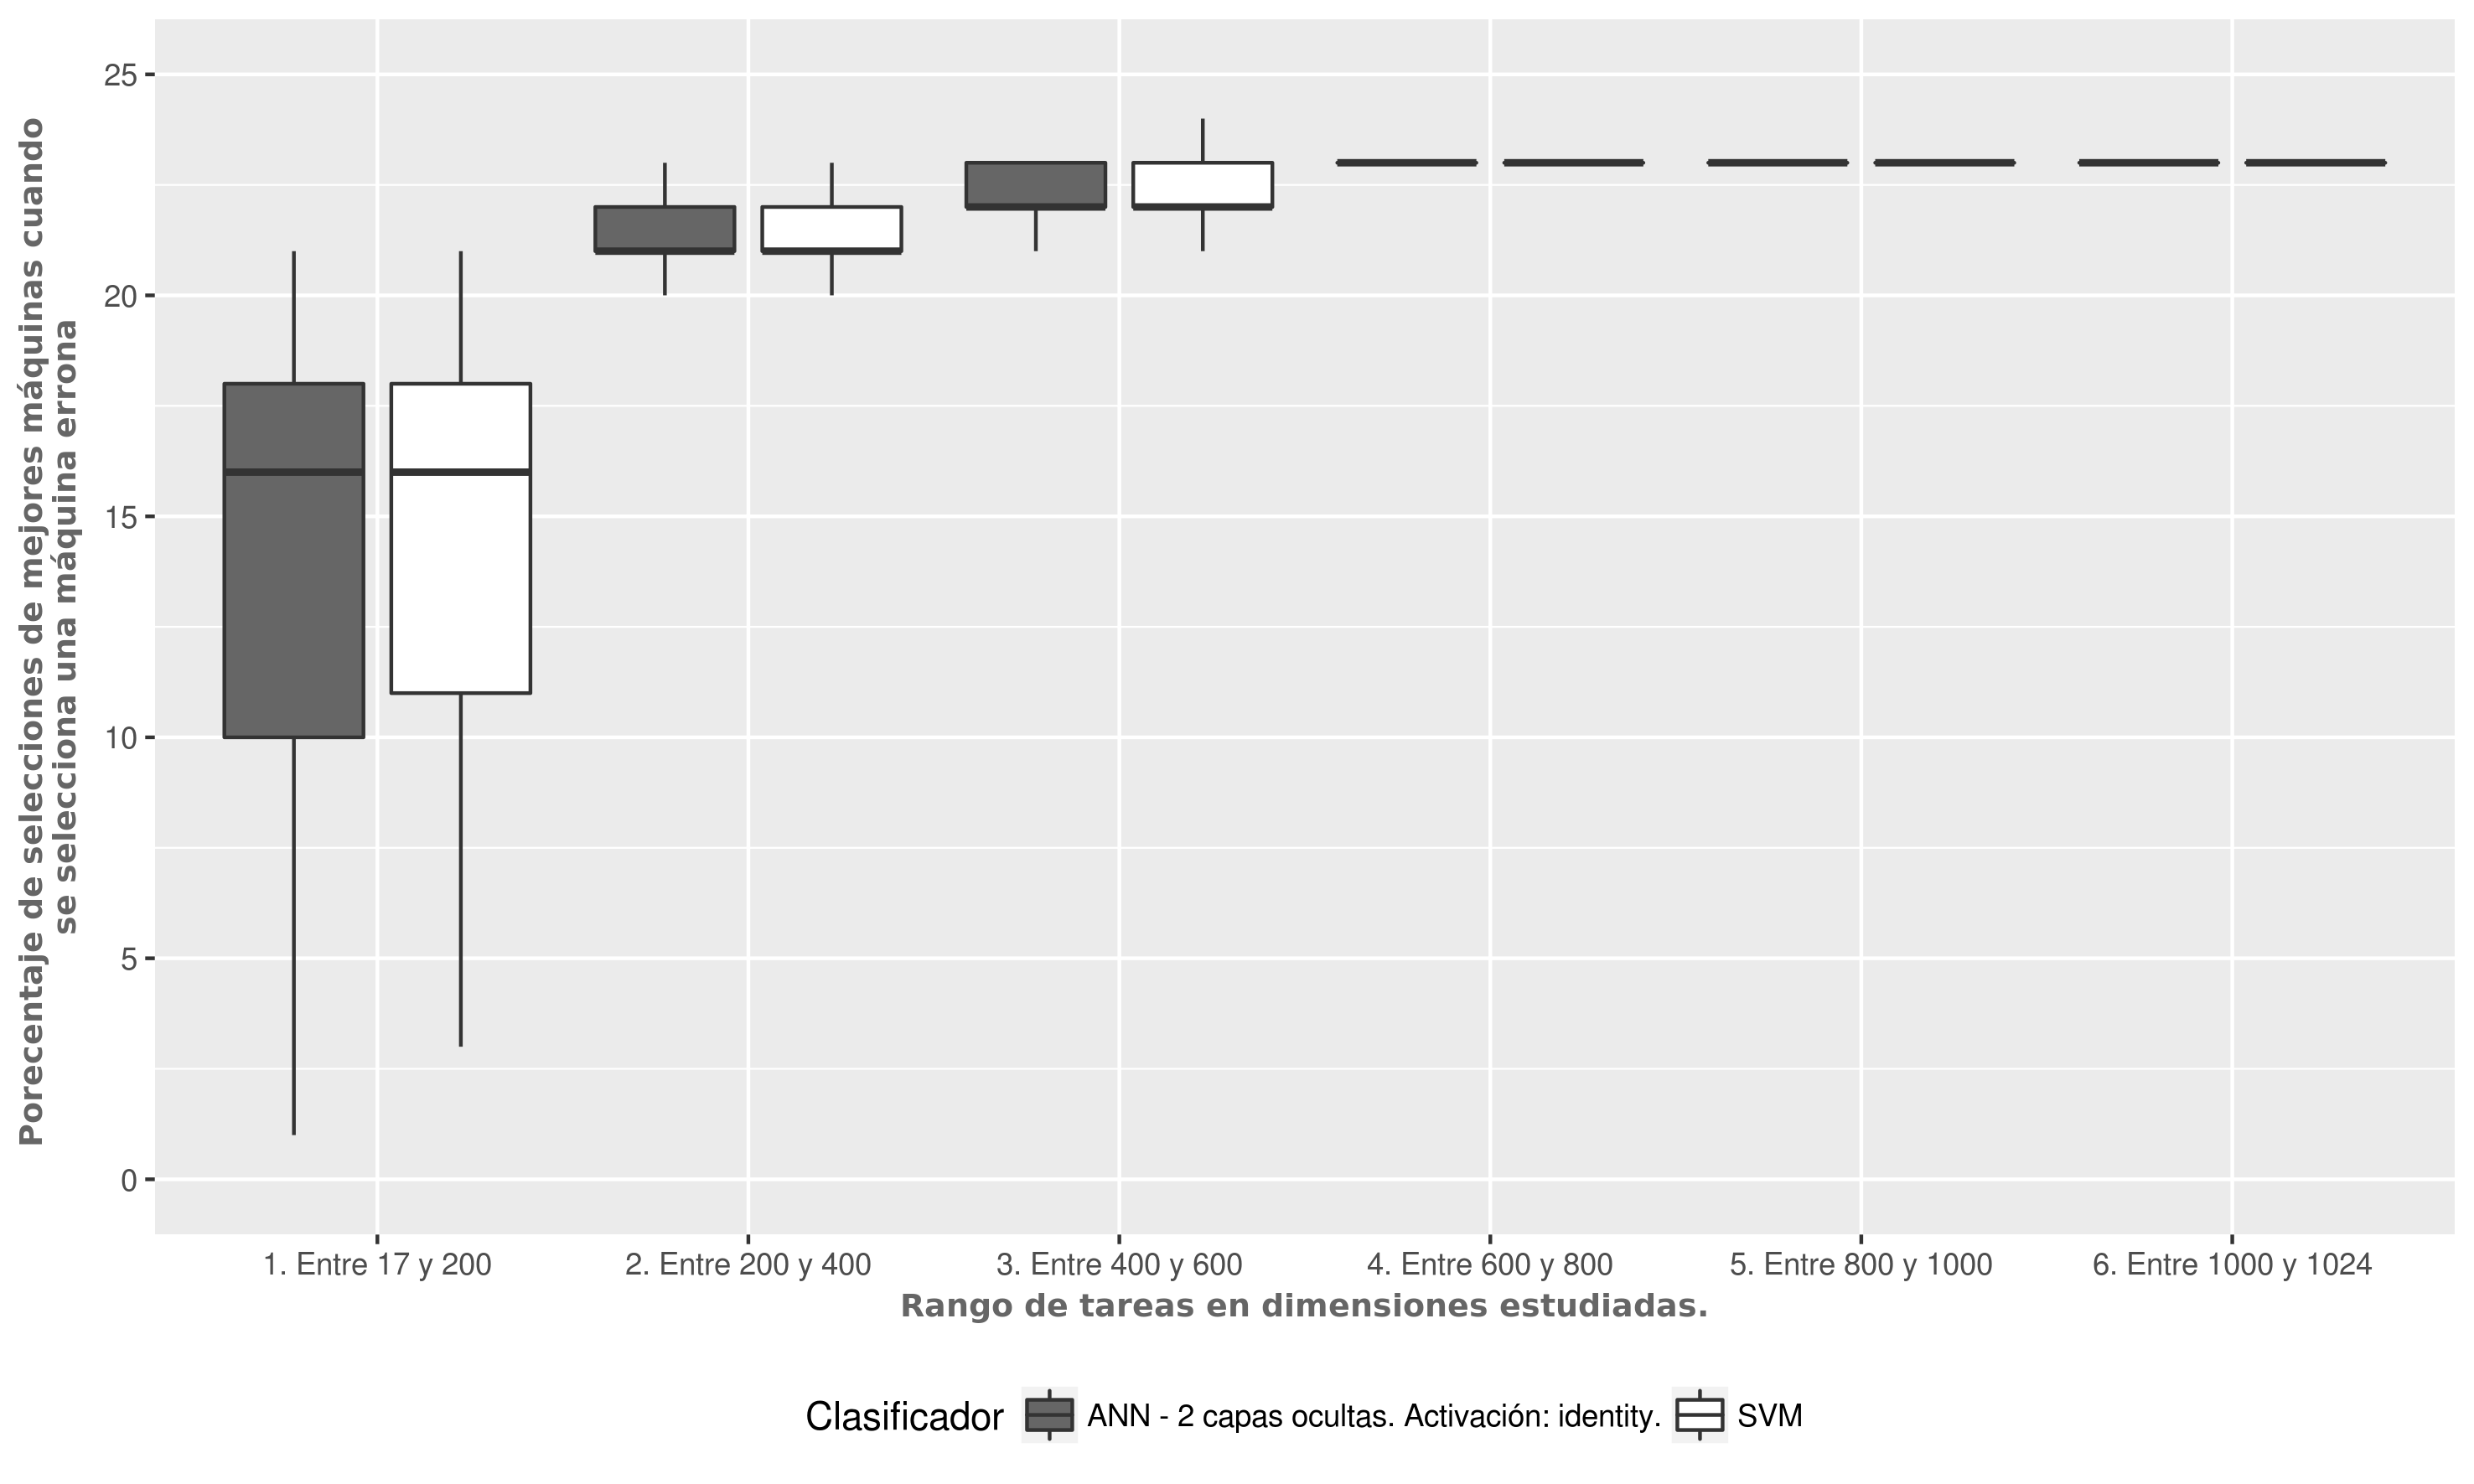
\includegraphics[width=\columnwidth]{imagenes/identity/4_porcentaje_maquinas_mejores_ann_2_capas_ocultas_identity.png}
  \caption{Porcentaje de selección de máquinas mejores frente a una selección diferente a la esperada para la red neuronal con activación \textit{identity} de dos capas ocultas y para la SVM.}
  \label{fig:identity_mejores}
\end{figure}

\section{Red neuronal con activación \textit{tanh} de dos capas ocultas}

La Figura \ref{fig:tanh_makespan} muestra las diferencias porcentuales de \textit{makespan} para la red neuronal con activación \textit{tanh} y para la SVM.
En esta se observa una leve mejora en \textit{makespan} para dimensiones grandes.
Esta mejora va acompañada de una mejora en la precisión, sustancial en comparación con las precisiones de las otras funciones de activación estudiadas, como se observa en la Figura \ref{fig:tanh_accuracy}.
 

\begin{figure}[H]
  \centering
  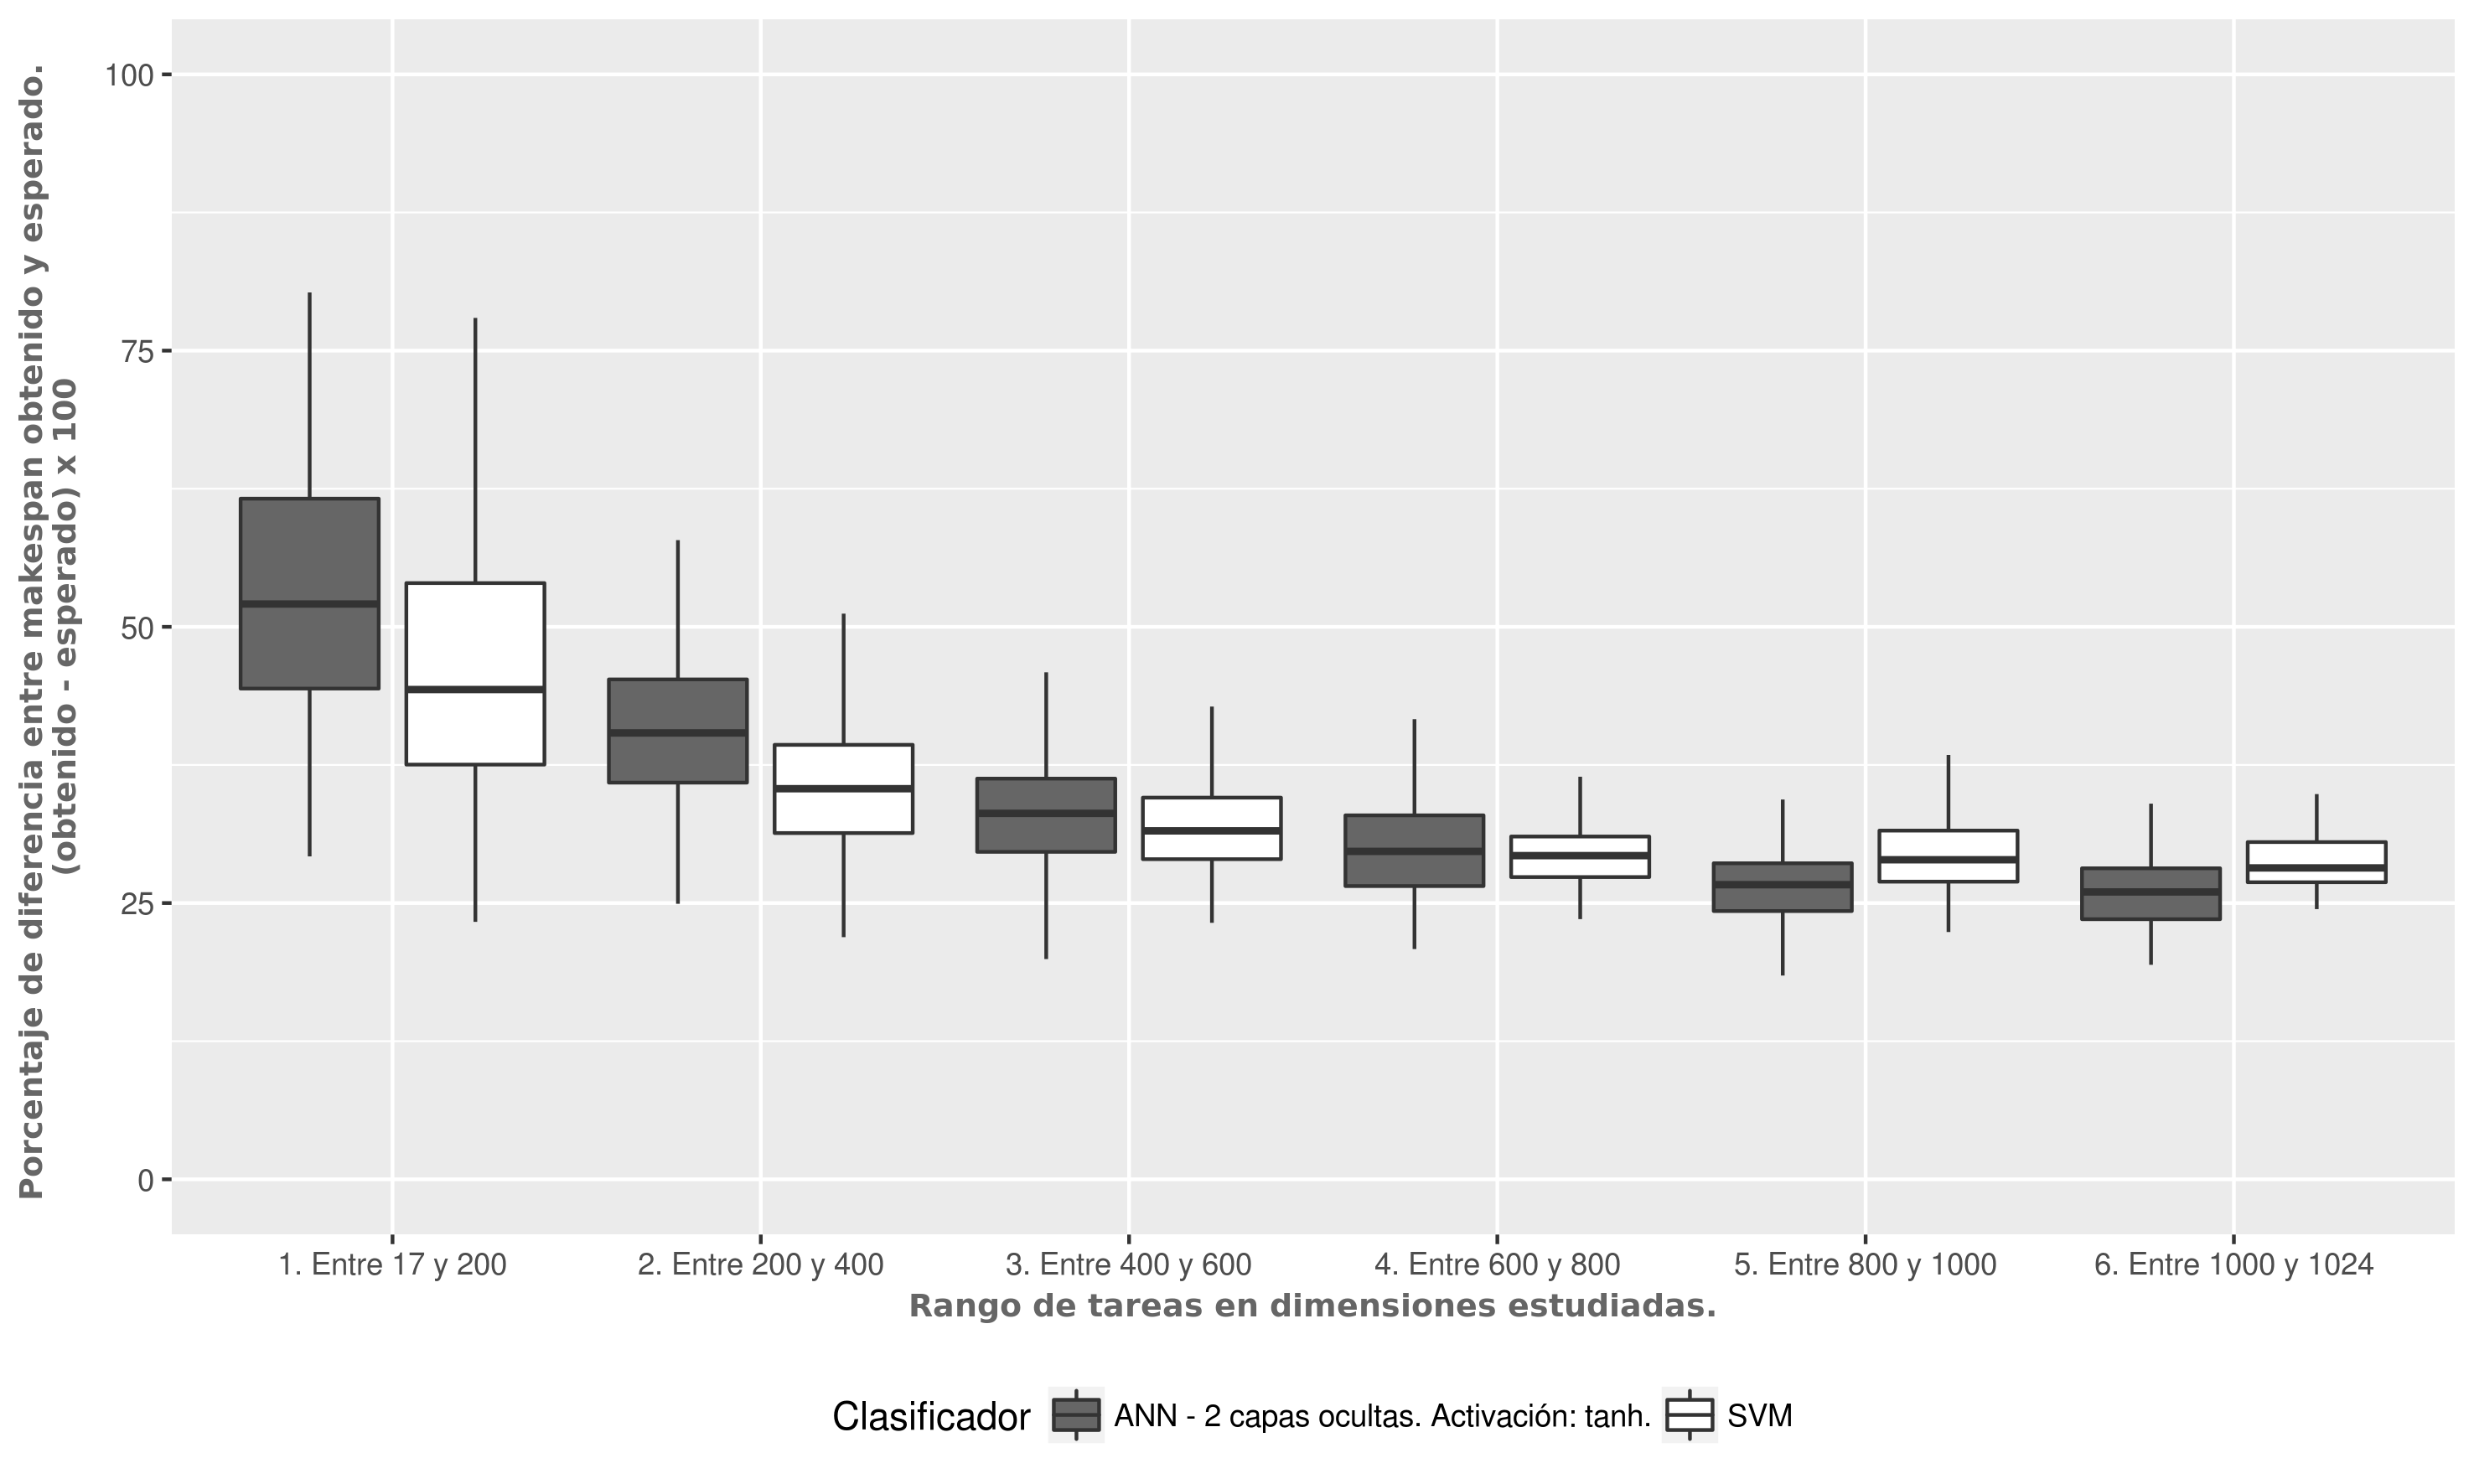
\includegraphics[width=\columnwidth]{imagenes/tanh/2_medianas_diferenciasann_2_capas_ocultas_tanh.png}
  \caption{Comparación de la diferencia porcentual de \textit{makespan} para la red neuronal con activación \textit{tanh}, de dos capas ocultas con respecto a los valores esperados obtenidos con el algoritmo Min-Min.
Así también se muestran los resultados obtenidos para la SVM.
Los resultados se muestran divididos en rangos de dimensión desde $ 17 \times 16$ a $ 1024 \times 16$}
  \label{fig:tanh_makespan}
\end{figure}

\begin{figure}[H]
  \centering
  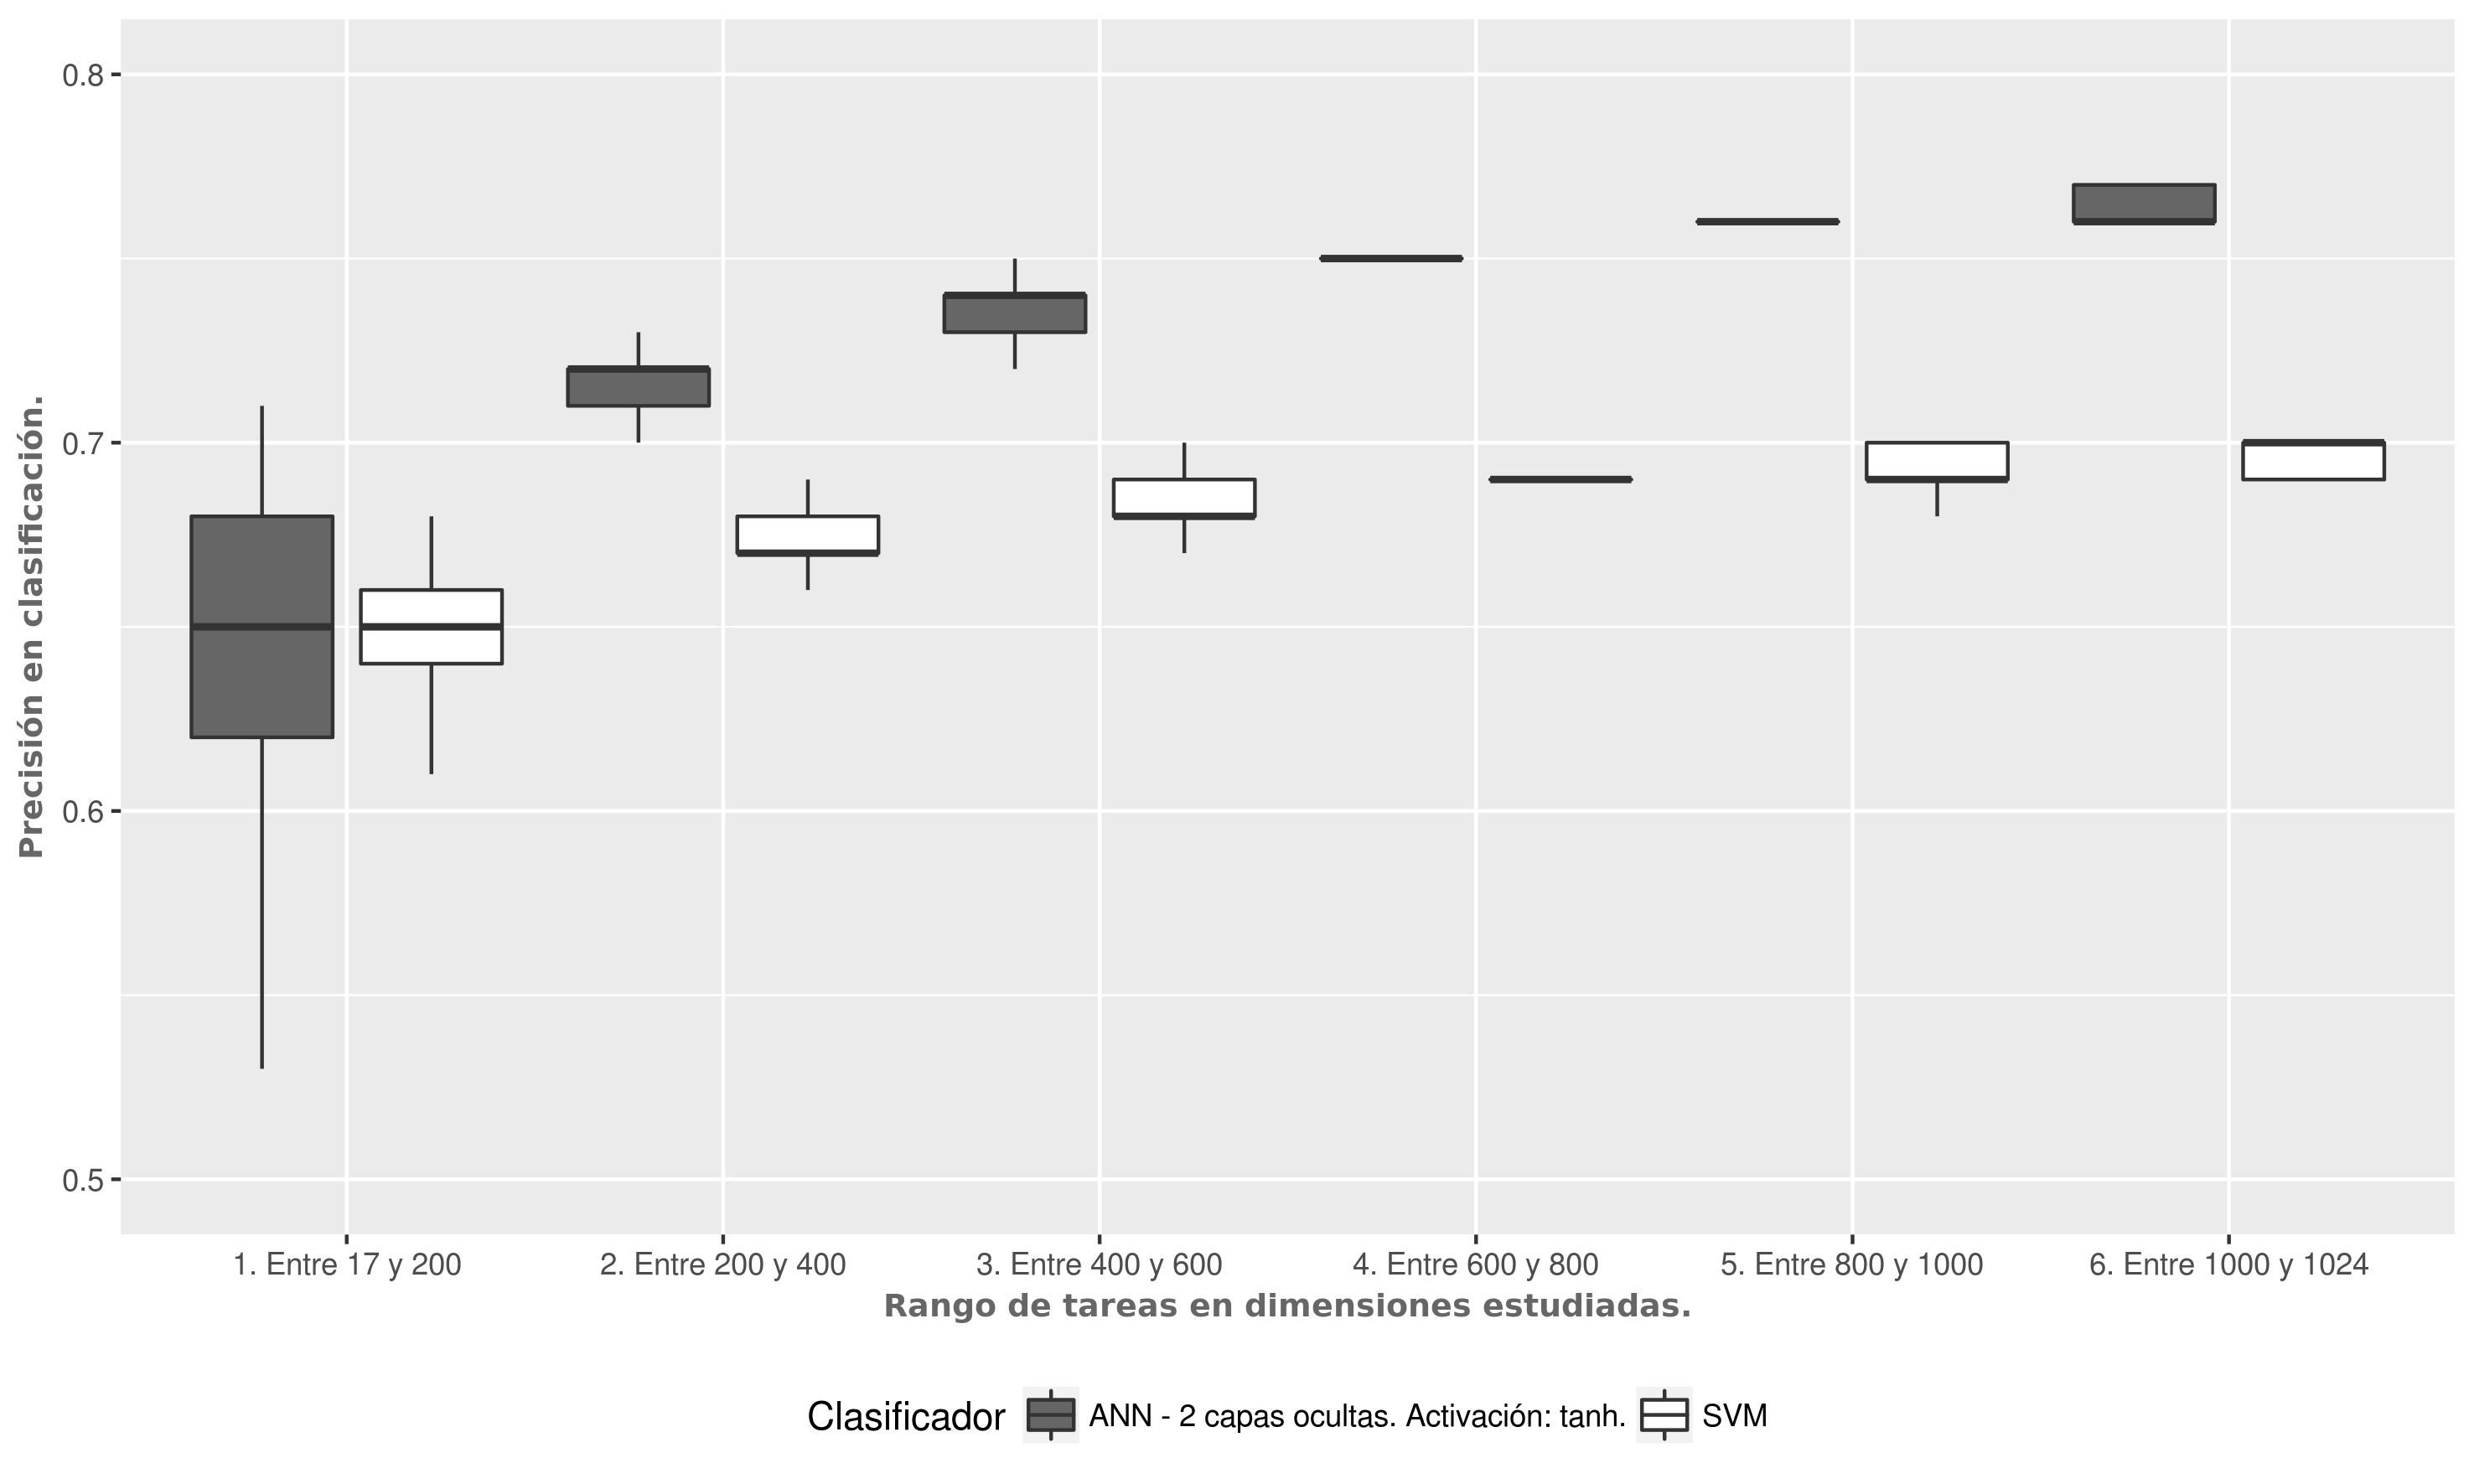
\includegraphics[width=\columnwidth]{imagenes/tanh/3_accuracy_ann_2_capas_ocultas_tanh.png}
  \caption{Precisión en clasificación para la red neuronal con función de activación \textit{tanh} y para la SVM.
Los resultados se muestran divididos en rangos de dimensión desde $ 17 \times 16$ a $ 1024 \times 16$.}
  \label{fig:tanh_accuracy}
\end{figure}

\paragraph{} Al estudiar las decisiones que se toman frente a un error en la selección de la máquina a la que una tarea es asignada, se encuentra que la red neuronal que utiliza la función de activación \textit{tanh} selecciona máquinas más lentas que la SVM.
Lo antedicho se observa en la Figura \ref{fig:tanh_mejores} 

\paragraph{} Para dimensiones grandes, se selecciona alrededor de un $15\%$ de mejores máquinas para esta función de activación, siendo este porcentaje el más bajo obtenido para todas las funciones de activación en esta dimensión del estudio.
Esto conduce a pensar que la precisión es fundamental para aproximarse al \textit{makespan} esperado y que las decisiones que se tomen a la hora de seleccionar una máquina diferente a la esperada pierden importancia frente a una precisión elevada en clasificación.
Esto parece ocurrir sobre todo en dimensiones grandes, donde un error puede costar caro en términos de tiempos de ejecución o \textit{makespan}.

\begin{figure}[H]
  \centering
  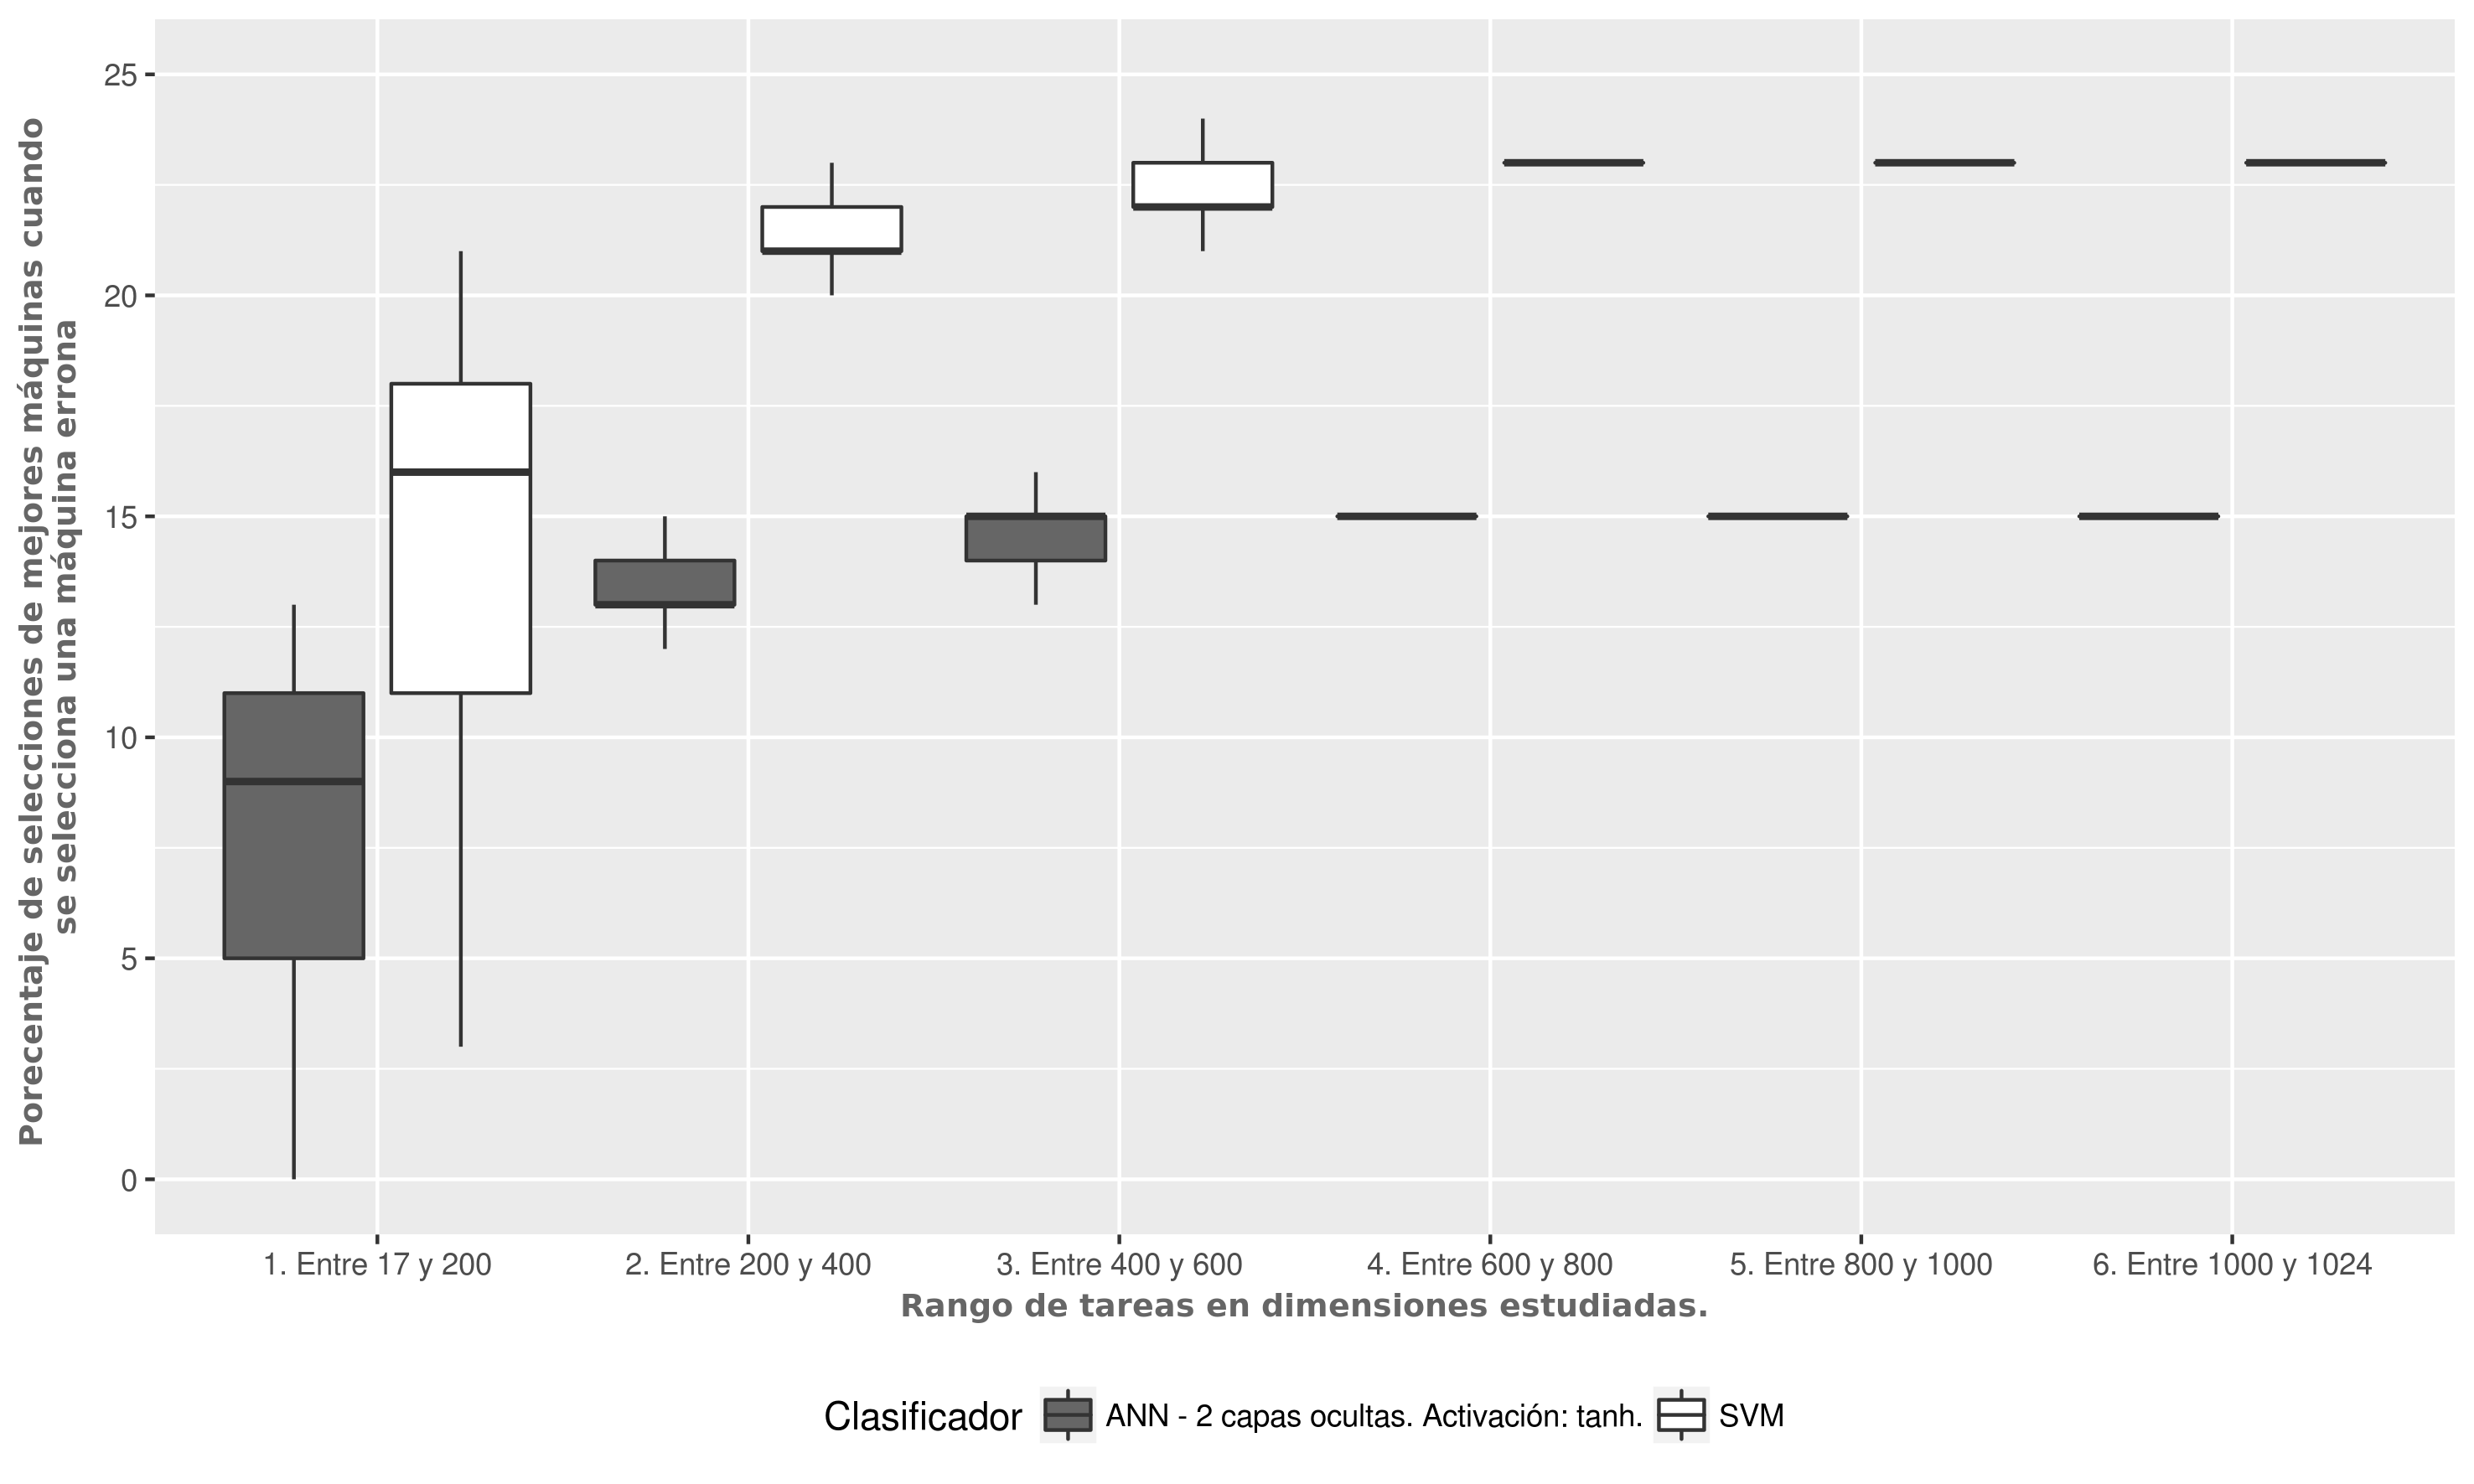
\includegraphics[width=\columnwidth]{imagenes/tanh/4_porcentaje_maquinas_mejores_ann_2_capas_ocultas_tanh.png}
  \caption{Porcentaje de selección de máquinas mejores frente a una selección diferente a la esperada para la red neuronal con activación \textit{tanh} de dos capas ocultas y para la SVM.}
  \label{fig:tanh_mejores}
\end{figure}

\section{Observaciones generales}

\paragraph{} En términos generales, entrenar redes neuronales con menor cantidad de capas ocultas, genera mejores resultados de \textit{makespan} en clasificación, que entrenar redes neuronales con mayor cantidad de capas ocultas.
Esto se traduce en mejores resultados de \textit{makespan} invirtiendo un menor tiempo de entrenamiento. 

\paragraph{} Para redes neuronales entrenadas utilizando \textit{tanh} e \textit{identity} como funciones de activación, el \textit{makespan} de los resultados mejora levemente con respecto al \textit{makespan} de los resultados obtenidos con SVM para dimensiones grandes del problema.
Se observa que hay una relación directa entre la precisión y la mejora porcentual de \textit{makespan}, así como también entre el porcentaje de selección de mejores máquinas frente a un error y la mejora porcentual de \textit{makespan}. 

\paragraph{} Los resultados obtenidos con la red neuronal con función de activación \textit{relu} no mejoran los resultados obtenidos con SVM en términos de \textit{makespan}, obteniendo precisiones en clasificación similares, teniendo un porcentaje menor de selección de mejores máquinas frente a un error. Esto hace que \textit{relu} sea una función de activación poco adecuada si el objetivo perseguido es aprender a resolver el problema HCSP.